% \iffalse meta-comment
%  rubiktwocube.dtx
% 
%  version v5.0  
%  February 25, 2018
%
%
%  Copyright 2018 
%  RWD Nickalls (dick@nickalls.org) and 
%  A Syropoulos (asyropoulos@yahoo.com)
%
% This work may be distributed and/or modified under the
% conditions of the LaTeX Project Public License, either version 1.3
% of this license or (at your option) any later version.
% The latest version of this license is in
%   http://www.latex-project.org/lppl.txt
% and version 1.3 or later is part of all distributions of LaTeX
% version 2005/12/01 or later.
%
%
% This work consists of the files rubiktwocube.dtx and rubiktwocube.ins
% and the derived file rubiktwocube.sty.
%
%<*readme>
%
% The rubikcube package provides a collection of LaTeX commands and macros 
% for the typesetting of Rubik cube configurations and rotation 
% sequences using the TikZ graphic language.
%
% Please report errors or suggestions for improvement to
%
%         Dick Nickalls or Apostolos Syropoulos
%
% This package requires the basic TikZ package to be loaded already
%</readme>
%
%<*driver>
\listfiles
\documentclass{ltxdoc}
\IfFileExists{rubiktwocube.sty}{\usepackage{rubiktwocube}}{%
    \GenericWarning{rubiktwocube.dtx}{Package file rubiktwocube.sty not found.
    Documentation will be messed up!^^J
    (Generate rubiktwocube.sty by (La)TeXing rubiktwocube.ins, and then^^J
    process rubiktwocube.dtx again)^^J}\stop
}%
\pagestyle{myheadings}
\markright{\texttt{rubiktwocube} \ \ (Rubik bundle v5.0, 2018) \ \ \texttt{www.ctan.org/pkg/rubik}}
\usepackage{rubikcube}  %% we require macros  @join and  rubikfont 
\usepackage{ifpdf}
\usepackage{url,path}     %% for references
\usepackage{supertabular} %% for Notation table
\usepackage{hypdoc}       %% for hyperref documenting of LaTeX packages
%%\OnlyDescription
\EnableCrossrefs
\PageIndex
\CodelineIndex
\CodelineNumbered
\RecordChanges
\setcounter{StandardModuleDepth}{1}
\begin{document}
  \DocInput{rubiktwocube.dtx}
  \PrintChanges
  \PrintIndex
\end{document}
%</driver>
% \fi
%
%
% 
%%% \CheckSum{2308} 
%
%%% \CharacterTable
%%  {Upper-case    \A\B\C\D\E\F\G\H\I\J\K\L\M\N\O\P\Q\R\S\T\U\V\W\X\Y\Z
%%   Lower-case    \a\b\c\d\e\f\g\h\i\j\k\l\m\n\o\p\q\r\s\t\u\v\w\x\y\z
%%   Digits        \0\1\2\3\4\5\6\7\8\9
%%   Exclamation   \!     Double quote  \"     Hash (number) \#
%%   Dollar        \$     Percent       \%     Ampersand     \&
%%   Acute accent  \'     Left paren    \(     Right paren   \)
%%   Asterisk      \*     Plus          \+     Comma         \,
%%   Minus         \-     Point         \.     Solidus       \/
%%   Colon         \:     Semicolon     \;     Less than     \<
%%   Equals        \=     Greater than  \>     Question mark \?
%%   Commercial at \@     Left bracket  \[     Backslash     \\
%%   Right bracket \]     Circumflex    \^     Underscore    \_
%%   Grave accent  \`     Left brace    \{     Vertical bar  \|
%%   Right brace   \}     Tilde         \~}
%
%
% \title{%
%       \ifpdf\pdfbookmark[1]{Title}{Title}\else\fi%
%        The \rubiktwocube\ package}
%
% \author{
%      RWD Nickalls (dick@nickalls.org) \\
%     A Syropoulos (asyropoulos@yahoo.com)
%       }
%  \date{This file describes version \RTCfileversion\ (\RTCfiledate)\\
%   \texttt{www.ctan.org/pkg/rubik}}
%  \maketitle
%
%  \begin{abstract}
%  The \rubiktwocube\ package provides LaTeX commands and macros 
%  for  typesetting  TwoCube (2x2x2) notation,  configurations, and 
%  rotation sequences  using the  TikZ graphic language. It is part of the 
%   Rubik `bundle'.
%  \end{abstract}
%
% 
% \begin{minipage}{12cm}
% \centering
% \ifpdf
%  \strut\hspace{5mm}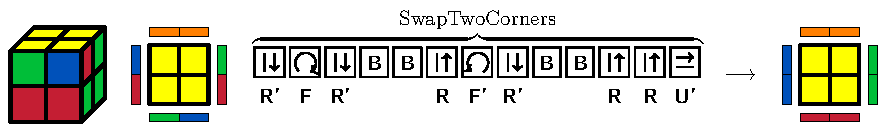
\includegraphics[width=12cm]{rubiktwo-doc-figA.pdf}
% \else
% \fi
% \end{minipage}
% 
%
%  \tableofcontents
%
% \pagebreak
%
% \section{Introduction}
%
% The  \rubiktwocube\  package (part of the \textsc{rubik} `bundle') provides  a 
% collection of \LaTeX\ commands 
% and macros for  typesetting  Rubik 2x2x2 cube  configurations  using the  
% PGF/TikZ graphic languages. 
% This package is a minor extension of the \textsc{rubikcube} package, and users are
% therefore  assumed to be familiar with  both the \textsc{rubikcube} and \textsc{rubikrotation}
%  packages. For examples of use see the file \texttt{rubikexamples.pdf}.
%
%
%      \subsection{Requirements}
%
%  The \rubiktwocube\ package requires the TikZ package (since it makes  
%  use  of the TikZ picture environment), and  also  the 
%  \textsc{rubikcube}   package.
%
%  For full functionality the complementary packages \textsc{rubikrotation}  and 
%  \textsc{rubikpatterns} also need to be loaded.
%  Note that the \textsc{rubikrotation}  package requires  Perl to be installed.
%  See  the `Installation' section in the \textsc{rubikcube} package documentation
% (\texttt{rubikcube.pdf}) for more  details.

% 
% 
%
%  \subsection{Copyright}
%  Copyright 2014--2018 RWD Nickalls and A Syropoulos.
%
% \medskip
% {\noindent}This work may be distributed and/or modified under the
% conditions of the LaTeX Project Public License, either
% version 1.3c of this license or any
% later version. The latest version of this licence is in 
%  |www.latex-project.org/lppl.txt|
%
%
% \section{Installation}
%
% The Rubik bundle consists of the four packages \textsc{rubikcube}, \textsc{rubikrotation},
% \textsc{rubikpatterns} and  \textsc{rubiktwocube}.
%
% Here we describe only the installation of the \textsc{rubiktwocube} package, 
% which  consists of the  following files:
%\begin{verbatim}
%   rubiktwocube.ins
%   rubiktwocube.dtx
%   rubiktwocube.pdf         --documentation of the rubiktwocube package
%   rubiktwo-doc-figA.pdf
%\end{verbatim}
% Before installing the \textsc{rubiktwocube} package make sure the following packages
% are already installed  (TikZ graphics system and the \textsc{rubikcube} package).
%
%
%  \subsection{\texttt{rubiktwocube.sty}}
%
%  The  style option \texttt{rubiktwocube.sty} is generated by  running (pdf)\LaTeX\ on  
% the file \texttt{rubiktwocube.ins}  as follows:
%\begin{verbatim}
%   pdflatex  rubiktwocube.ins 
%\end{verbatim}
%
%
%  \subsection{\texttt{rubiktwocube.pdf}}
%
% The documentation file (\texttt{rubiktwocube.pdf}) is then generated using the following
% steps\,\footnote{Several pdflatex runs are required, since the documentation includes 
% an index as well as hyperef links (the package \texttt{hypdoc}
% is used). Prior to the first run it is
% a good idea to delete any relevant \texttt{.toc}, \texttt{.aux}, \texttt{.out} files.}:
%\begin{verbatim}
%   pdflatex   rubiktwocube.dtx
%   pdflatex   rubiktwocube.dtx
%   makeindex -s gind.ist  rubiktwocube
%   makeindex -s gglo.ist -o rubiktwocube.gls  rubiktwocube.glo
%   pdflatex   rubiktwocube.dtx
%   pdflatex   rubiktwocube.dtx
%\end{verbatim}
%
%
%  \subsection{Placing the files}
%
% Place the files either in the local working directory, or where your system 
% will find them. For a Linux system with a standard \TeX\ Directory Structure (TDS), then:
%
%\medskip
%{\noindent}*.sty  $\rightarrow$ 
%   \texttt{/usr/local/texlive/texmf-local/tex/latex/rubik/}
%{\newline}*.pdf  $\rightarrow$  \texttt{/usr/local/texlive/texmf-local/doc/rubik/}
%
% \medskip
% {\noindent}Finally, (depending on your system) update the  \TeX\ file database.
% For~example, on a Linux system one uses the  \texttt{texhash} command.
%
%
% \subsection{Usage}
%
% Load the package by using the command \cmd{\usepackage\{rubiktwocube\}}.
% Note that the \rubiktwocube\ package requires the TikZ package, and so always load TikZ 
% before \rubiktwocube\  as follows:
% \begin{quote}
%\begin{verbatim}
% \usepackage{tikz}
% \usepackage{rubikcube,rubikrotation,rubikpatterns,rubiktwocube}
%\end{verbatim}
% \end{quote}
%
%
%
%  \subsection{\texttt{rubikexamples.pdf}}
%
% The Rubik bundle includes a  `RubikExamples' file (\texttt{rubikexamples.pdf})
% as well as associated  \texttt{.sh} (Linux) and \texttt{.bat} (Microsoft) batch 
% files which can be used to facilitate processing the source file (\texttt{rubikexamples.tex}). 
% See  the `Installation' section in the \textsc{rubikcube} package documentation
% (\texttt{rubikcube.pdf}) for details regarding processing the  examples source file.
%
%
%
%  \pagebreak
%
%        \section{Command conventions}
%        \label{sec:conventions}
%
%  The examples given in  the file \texttt{rubikexamples.pdf} present a good overview of 
%  the commands and how to use them.
% 
%
%
%   \subsection[Keywords Two and Rubik]{The keywords Two and Rubik in commands}
%
% In order to try and keep commands intuitive\,\footnote{This is a tricky problem 
% given the large number of commands, so any  feedback or  ideas on how to avoid ambiguity, 
% including  pruning or revising `bad' commands, is always welcome.} 
% we adopt the convention that  the word `Two' in a command  reflects the fact that 
% the command  relates to a 2x2x2 cube (a `Two' cube). Similarly, commands which relate 
% to a 3x3x3 cube (a `Rubik' cube) ---see the \textsc{rubikcube} package--- 
% use instead the word `Rubik'. 
%
%
%
% It is assumed that users are familiar with the \textsc{rubikcube} 
% and \textsc{rubikrotation} packages, since virtually all \rubiktwocube\  
% commands  mirror  the Rubik (3x3x3) cube commands, such that  the word  `Rubik'  
% is  replaced by the word `Two' (exceptions are highlighted). 
% For example, the commands for drawing a 2x2x2 cube  and a 3x3x3 cube from a RU viewpoint
% are respectively \cmd{\DrawTwoCubeRU} and \cmd{\DrawRubikCubeRU}.
%  The examples given in  the file \texttt{rubikexamples.pdf} present a good overview of 
% the commands and how to use them.
%
%  For more detailed information see (a)~the `code' section (Section~\ref{sec:thecode}), 
%  or (b)~see the equivalent  3x3x3 commands in the \textsc{rubikcube} package.
%
%
%
%
%
%  \section{Colour commands}
%   \label{sec:listofcolourcommands}
%
% The following  list  shows the \rubiktwocube\  colour commands  paired 
% (for convenience) with the equivalent 3x3x3 version from the 
% \textsc{rubikcube} package. The \texttt{..} indicates that mandatory arguments are required.
%
% 
%\begin{verbatim}
%  RubikCube           TwoCube
%  3x3x3               2x2x2
%
% \RubikCubeSolved       \TwoCubeSolved
% \RubikCubeSolvedWY     \TwoCubeSolvedWY
% \RubikCubeSolvedWB     \TwoCubeSolvedWB
% \RubikCubeGrey         \TwoCubeGrey
% \RubikCubeGray         \TwoCubeGray
% \RubikCubeGreyWY
% \RubikCubeGrayWY
% \RubikCubeGreyWB
% \RubikCubeGrayWB
% \RubikCubeGreyAll      \TwoCubeGreyAll
% \RubikCubeGrayAll      \TwoCubeGrayAll
% \RubikSolvedConfig..   \TwoSolvedConfig..
%
% \RubikFaceUp..         \TwoFaceUp..
% \RubikFaceDown..       \TwoFaceDown..
% \RubikFaceLeft..       \TwoFaceLeft..
% \RubikFaceRight..      \TwoFaceRight..
% \RubikFaceFront..      \TwoFaceFront..
% \RubikFaceBack..       \TwoFaceBack..
% \RubikFaceUpAll..      \TwoFaceUpAll..
% \RubikFaceDownAll..    \TwoFaceDownAll..
% \RubikFaceLeftAll..    \TwoFaceLeftAll..
% \RubikFaceRightAl..    \TwoFaceRightAll..
% \RubikFaceFrontAl..    \TwoFaceFrontAll..
% \RubikFaceBackAll..    \TwoFaceBackAll..
%
% \RubikSidebarWidth..   \TwoSidebarWidth..          
% \RubikSidebarLength..  \TwoSidebarLength..          
% \RubikSidebarSep..     \TwoSidebarSep..          
%
% \RubikSliceTopL..      \TwoSliceTopL..
% \RubikSliceTopR..      \TwoSliceTopR..
% \RubikSliceBottomL..   \TwoSliceBottomL..
% \RubikSliceBottomR..   \TwoSliceBottomR..
%\end{verbatim}
%
%
%
%  \section{Draw commands}
%   \label{sec:listofdrawcommands}
%
% The following  list  shows the \rubiktwocube\  Draw commands  paired 
% (for convenience) with the equivalent 3x3x3 version from the 
% \textsc{rubikcube} package. Commands in round brackets show short-hand 
% equivalents.
%
%
%\begin{verbatim}
%  RubikCube               TwoCube
%  3x3x3                   2x2x2
%
% \DrawRubikCubeRU         \DrawTwoCubeRU
% \DrawRubikCubeRD         \DrawTwoCubeRD
% \DrawRubikCubeLU         \DrawTwoCubeLU
% \DrawRubikCubeLD         \DrawTwoCubeLD
% \DrawRubikCubeF          \DrawTwoCubeF
% \DrawRubikCubeSF         \DrawTwoCubeSF
%
% \DrawRubikCubeSidebarFL..  \DrawTwoCubeSidebarFL..
% \DrawRubikCubeSidebarFR..  \DrawTwoCubeSidebarFR..
% \DrawRubikCubeSidebarFU..  \DrawTwoCubeSidebarFU..
% \DrawRubikCubeSidebarFD..  \DrawTwoCubeSidebarFD..
% \DrawRubikCubeSidebarBL..  \DrawTwoCubeSidebarBL..
% \DrawRubikCubeSidebarBR..  \DrawTwoCubeSidebarBR..
% \DrawRubikCubeSidebarBU..  \DrawTwoCubeSidebarBU..
% \DrawRubikCubeSidebarBD..  \DrawTwoCubeSidebarBD..
%
% \DrawRubikFaceUp         \DrawTwoFaceUp         (= \DrawTwoFaceU )
% \DrawRubikFaceDown       \DrawTwoFaceDown       (= \DrawTwoFaceD )
% \DrawRubikFaceLeft       \DrawTwoFaceLeft       (= \DrawTwoFaceL )
% \DrawRubikFaceRight      \DrawTwoFaceRight      (= \DrawTwoFaceR )
% \DrawRubikFaceFront      \DrawTwoFaceFront      (= \DrawTwoFaceF )
% \DrawRubikFaceBack       \DrawTwoFaceBack       (= \DrawTwoFaceB )
%
% \DrawRubikFaceUpSide     \DrawTwoFaceUpSide     (= \DrawTwoFaceUS )
% \DrawRubikFaceDownSide   \DrawTwoFaceDownSide   (= \DrawTwoFaceDS )
% \DrawRubikFaceLeftSide   \DrawTwoFaceLeftSide   (= \DrawTwoFaceLS )
% \DrawRubikFaceRightSide  \DrawTwoFaceRightSide  (= \DrawTwoFaceRS )
% \DrawRubikFaceFrontSide  \DrawTwoFaceFrontSide  (= \DrawTwoFaceFS )
% \DrawRubikFaceBackSide   \DrawTwoFaceBackSide   (= \DrawTwoFaceBS )
%
% \DrawRubikFlatUp..       \DrawTwoFlatUp..
% \DrawRubikFlatDown..     \DrawTwoFlatDown..
% \DrawRubikFlatLeft..     \DrawTwoFlatLeft..
% \DrawRubikFlatRight..    \DrawTwoFlatRight..
% \DrawRubikFlatFront..    \DrawTwoFlatFront..
% \DrawRubikFlatBack..     \DrawTwoFlatBack..
%
%\end{verbatim}
%
%
%
%
%  \section{Rotation commands}
%   \label{sec:rotationcommands}
%
%  \bigskip
%
%
%\begin{verbatim}
%  RubikCube           TwoCube
%  3x3x3               2x2x2
%
% \RubikRotation..     \TwoRotation..
% \SaveRubikState..    \SaveTwoState..
% \ShowErrors          \ShowErrors
% \CheckState          \CheckState
%\end{verbatim}
%
%
%  \subsection{List of rotation commands}
%   \label{sec:listofrotationcommands}
%
%
% All the commands presented here also have a \cmd{\Two\{\}} equivalent form which 
% typesets both the hieroglyph and its lettercode in a vertical format. 
% These have been omitted  here owing to the difficulty of including this form easily 
% in the following table.
%
% 2x2x2 \textsc{changes}: Note that all these command names mirror their 3x3x3 equivalents in 
% the \textsc{rubikcube} package; the changes in the command prefixes 
% are as follows: 
%
% \cmd{\tr} $\leftarrow$ \cmd{\rr}
%
% \cmd{\trh} $\leftarrow$ \cmd{\rrh}
%
% \cmd{\Two} $\leftarrow$ \cmd{\Rubik}
%
% \cmd{\textTwo} $\leftarrow$ \cmd{\textRubik}
%
% \pagebreak
%
%  \subsubsection{Face rotations}
%   \label{sec:facerotations}
%
%
%  \newcommand{\dnstrut}{\rule{0pt}{17pt}}
%  \newcommand{\dns}{\hspace{2mm}}
%  \newcommand{\dnsp}{\hspace{2mm}} 
%
%  \newcommand{\dnTwo}[1]{%
%    \dnstrut\tr{#1}\dns\cmd{\tr\{#1\}}%
%    & \trh{#1}\dns\cmd{\trh\{#1\}}%
%    & \Two{#1}\dns\cmd{\Two\{#1\}} \nonumber\\%
%    }%  
%
%  \newcommand{\dntextTwo}[1]{%
%   \dnstrut\tr{#1}\dns\cmd{\tr\{#1\}}%
%   & \trh{#1}\dns\cmd{\trh\{#1\}}%
%   & \textTwo{#1}\dns\cmd{\textTwo\{#1\}} \nonumber\\%
%   }%
%
%
%  \begin{supertabular}[lll]{p{3cm} p{3cm} p{4.5cm}}
%   \dntextTwo{U}
%   \dntextTwo{Up}
%   \dntextTwo{D}
%   \dntextTwo{Dp}
%   \dntextTwo{L}
%   \dntextTwo{Lp}
%   \dntextTwo{R}
%   \dntextTwo{Rp}
%   \dntextTwo{F}
%   \dntextTwo{Fp}
%   \dntextTwo{B}
%   \dntextTwo{Bp}
%  \end{supertabular}
%
%
%
%    \subsubsection{Axis rotations}
%     \label{sec:listofaxisrotations}
%
%  \begin{supertabular}[lll]{p{3cm} p{3cm} p{4.5cm}}
%   \dnTwo{x}
%   \dnTwo{xp}
%   \dnTwo{y}
%   \dnTwo{yp}
%   \dnTwo{z}
%   \dnTwo{zp}
%  \end{supertabular}
%
%
%  \begin{supertabular}[lll]{p{3cm} p{3cm} p{4.5cm}}
%   \dnTwo{u}
%   \dnTwo{up}
%   \dnTwo{d}
%   \dnTwo{dp}
%   \dnTwo{l}
%   \dnTwo{lp}
%   \dnTwo{r}
%   \dnTwo{rp}
%   \dnTwo{f}
%   \dnTwo{fp}
%   \dnTwo{b}
%   \dnTwo{bp}
%  \end{supertabular}
%
%
%  \begin{supertabular}[lll]{p{3cm} p{3cm} p{4.5cm}}
%   \dnTwo{Uc}
%   \dnTwo{Ucp}
%   \dnTwo{Dc}
%   \dnTwo{Dcp}
%   \dnTwo{Lc}
%   \dnTwo{Lcp}
%   \dnTwo{Rc}
%   \dnTwo{Rcp}
%   \dnTwo{Fc}
%   \dnTwo{Fcp}
%   \dnTwo{Bc}
%   \dnTwo{Bcp}
%  \end{supertabular}
%
%
%  \begin{supertabular}[lll]{p{3cm} p{3cm} p{4.5cm}}
%   \dnTwo{CR}
%   \dnTwo{CRp}
%   \dnTwo{CL}
%   \dnTwo{CLp}
%   \dnTwo{CU}
%   \dnTwo{CUp}
%   \dnTwo{CD}
%   \dnTwo{CDp}
%   \dnTwo{CF}
%   \dnTwo{CFp}
%   \dnTwo{CB}
%   \dnTwo{CBp}
%  \end{supertabular}
%
%
%
%    \section{References}
%  
%  See the \textsc{rubikcube} package documentation for a full list of references.  
%
%
%    \section{Change history}
% 
% \begin{itemize}
%
% \item Version 5.0 (February 2018)
%
%  ---First release.
%
% \end{itemize}
%  
%
%
%
% ^^A =======================
% \StopEventually{\PrintIndex}
%
% \bigskip\bigskip\bigskip\bigskip
%
% \section{The code} 
%   \label{sec:thecode}
%  
%  All the 2x2x2 code here is essentially a  cut-down version of the  
%  3x3x3  code (\textsc{rubikcube} package); i.e.,~we have mostly just 
%  removed the 3x3x3 code relating to middle columns and rows, exchanged the 
%  word `Rubik' for the word `Two' in command names, and refashioned some of the commands 
%  involved in writing the  temporary file \texttt{rubikstate.dat}.
%  We assume that users are familiar with the \textsc{rubikcube} and 
%  \textsc{rubikrotation} package  documentation.
%
%  In order to avoid much repetition,  we describe here only the 
%  essential details for understanding the relatively minor changes made in order to 
%  transform the earlier 3x3x3  \textsc{rubikcube} package code into 
%  working 2x2x2 code. In the following, the various instances of the 
%  heading `\textsc{changes:}' imply that more extensive details will be found 
%  with the equivalent `Rubik' commands in  the \textsc{rubikcube} or \textsc{rubikrotation} 
%  package documentation.
%
%  Relatively  few 2x2x2 square hieroglyphs are required; some needed
%  reformulating  from their 3x3x3 cousins, ie those associated 
%  with  \texttt{L,\,Lp,\,R,\,Rp,\,U,\,Up,\,D,\,Dp}. 
%  The axis rotations and the rotations \texttt{F,\,Fp,\,B,\,Bp}  simply required 
%  renaming; for~example, as a `TwoRotationHieroglyph' (\cmd{\trh..}) instead of 
%  the 3x3x3 `RubikRotationHieroglyph (\cmd{\rrh..}).   
%
%
%
%
%   \subsection{Package heading}
% 
% The `RTC' in the following refers to the package name RubikTwoCube.
%
%    \begin{macrocode}
%<*rubiktwocube>
\def\RTCfileversion{5.0}%
\def\RTCfiledate{2018/02/25}% February 25, 2018
\NeedsTeXFormat{LaTeX2e}
\ProvidesPackage{rubiktwocube}[\RTCfiledate\space (v\RTCfileversion)]
%    \end{macrocode}
%  The package requires TikZ (we use the  pgfmathsetmacro command)
%  ---so we load it if not already loaded.
%    \begin{macrocode}
\@ifpackageloaded{tikz}{}{%
  \typeout{---rubiktwocube requires the TikZ package.}%
  \RequirePackage{tikz}}%
%    \end{macrocode}
%
%
%
% {\noindent}The package requires \texttt{rubikcube.sty}. However \texttt{rubikcube.sty}
% is not automatically loaded (for the moment at least) since this makes it difficult 
% to errorcheck new versions, so we just write a message.
%    \begin{macrocode}
\@ifpackageloaded{rubikcube}{}{%
   \typeout{---rubiktwocube requires the rubikcube package.}%
   }%
\@ifpackageloaded{rubikrotation}{}{%
   \typeout{---rubiktwocube requires the rubikrotation package.}%
   }%
%    \end{macrocode}
%
%    \begin{macro}{\rubiktwocube}
%  First we create a suitable logo
%    \begin{macrocode}
\newcommand{\rubiktwocube}{\textsc{rubiktwocube}}%
%    \end{macrocode}
%    \end{macro}
%
%
%
%
%    \subsection{Saving the Two-cube state}
%    \label{sec:codesavingtwostate}
%
% Note that this package   writes  this state data to the same `output' file 
% (\texttt{rubikstate.dat}) as used by the 3x3x3 \textsc{rubikrotation} package, 
% since there is no need to change this (since the TwoCube corners will be processed in
% exactly the same way as for 3x3x3 cube corners).
%
%    \begin{macro}{\@printTWOstate}
%  This internal command  writes the TwoCube  state data to
%  the  `output' file \texttt{rubikstate.dat}, and is used by the \cmd{\TwoRotation} command
%  (see  also \textsc{rubikrotation} package documentation  Sections on \textit{save rubikstate} 
%  and \textit{general overview} for further details).
%  The file \texttt{rubikstate.dat} is read by the Perl script, and represents 
%  the state on which the  \cmd{\TwoRotation} command acts.
% 
%  \textsc{changes}: Since this is a TwoCube all the non-corner facelets 
%  (ie those in middle rows \& columns) are filled with X (grey). 
%  We have also introduced a new line  in the output file (\texttt{rubikstate.dat})
%  namely \texttt{cubesize,two} which is used to inform the Perl program  that we 
%  are dealing with a TwoCube. 
%    \begin{macrocode}
\newcommand{\@printTWOstate}{%
   \@print{cubesize,two}%
   \@print{\space \space up,\Ult,\Umt,\Urt,\Ulm,\Umm,\Urm,\Ulb,\Umb,\Urb}%
   \@print{down,\Dlt,\Dmt,\Drt,\Dlm,\Dmm,\Drm,\Dlb,\Dmb,\Drb}%
   \@print{left,\Llt,\Lmt,\Lrt,\Llm,\Lmm,\Lrm,\Llb,\Lmb,\Lrb}%
   \@print{right,\Rlt,\Rmt,\Rrt,\Rlm,\Rmm,\Rrm,\Rlb,\Rmb,\Rrb}%
   \@print{front,\Flt,\Fmt,\Frt,\Flm,\Fmm,\Frm,\Flb,\Fmb,\Frb}%
   \@print{back,\Blt,\Bmt,\Brt,\Blm,\Bmm,\Brm,\Blb,\Bmb,\Brb}%
}
%    \end{macrocode}
%    \end{macro}
%
%
%
%
%    \subsection{SaveTwoState command}
%    \label{sec:codesavetwostate}
%
%    \begin{macro}{\SaveTwoState}
% We create  a TwoCube version of the existing \cmd{\SaveRubikState} command 
% (\textsc{rubikrotation} package), simply for symmetry and  convenience. 
% This command  is identical to the `Rubik' version, and will require 
% the \textsc{rubikrotation} package to be loaded already (as does the following 
% \cmd{\TwoRotation} command.
%    \begin{macrocode}
\newcommand{\SaveTwoState}{\SaveRubikState}
%    \end{macrocode}
%    \end{macro}
%
%
%
%
%    \subsection{TwoRotation command}
%    \label{sec:codetworotation}
%
% Note that this command writes the data to the same file 
% (\texttt{rubikstate.dat}) as that output  by the  equivalent 3x3x3 
% \cmd{\RubikRotation} command,  since there is no need to change this.
%
%  Note that although the system works perfectly well even if we just continue to use the 
%  3x3x3 \cmd{\RubikRotation} command, it was felt appropriate  to implement  a special 
%  TwoCube version  of this command, since this allows  the Perl script to  be aware 
%  (via the \texttt{cubesize,two} line written to the \texttt{rubikstate.dat} file) 
%  which sort of cube it is dealing with, and hence allows the option for the program to
%  adjust its action accordingly (for example, with regard to the randomisation procedure 
%  which is different for different cubes).
%  
%
%    \begin{macro}{\TwoRotation}
% The \cmd{\TwoRotation}\oarg{integer}\marg{comma separated sequence} 
% command (a)~writes the current TwoCube state to the file \texttt{rubikstate.dat},
% (b)~writes the rotation sequence (either once or multiple times depending 
% on the value of the optional integer argument), and then (c)~CALLs the 
% Perl script \texttt{rubikrotation.pl}.  It~also writes comments to the 
% data file and also to the log file.
%
% The way we allow the user to (optionally) process the main argument multiple
%  times  is simply by writing the associated output command multiple
% times to the output data-file. Consequently, we require the \cmd{\TwoRotation} 
% command to allow a square-bracket optional
% argument (a non-negative integer) to specify the number of such repeats.
%
% \textsc{2x2x2 changes}: (1)~We have  replaced `Rubik' by `Two' in the command-name 
% (2)~we use the command \cmd{\@printTWOstate} (see above) to write the current state data,
% (3)~the \texttt{RTC} in the fileversion and filedate names denotes  `RubikTwoCube'.
%    \begin{macrocode}
\newcommand{\TwoRotation}[2][1]{%
   \typeout{---TeX process}%
   \typeout{---script = TwoRotation cmd (rubiktwocube.sty)%
                         v\RTCfileversion\space (\RTCfiledate)}%
   \typeout{---NEW rotation command}%
   \typeout{---command = TwoRotation[#1]{#2}}%
   \typeout{---writing current TWOcube state to file rubikstate.dat}%
   \@openstatefile% open data file
   \@print{\@comment filename: rubikstate.dat}%
   \@print{\@comment written by TwoRotation cmd (rubiktwocube.sty)%
                              v\RTCfileversion\space (\RTCfiledate)}%
   \@printTWOstate%
   %% countingloop code from Feuersaenger (2015)
   \newcount\ourRRcounter%
   \@countingloop{\ourRRcounter} in 1:{#1}{%
         \immediate\write\outfile{rotation,#2}}%
   \@closestatefile% close data file
   \typeout{---CALLing Perl script (rubikrotation.pl)}%
   \immediate\write18{\rubikperlcmd}%
   \typeout{---inputting NEW datafile (data written by Perl script)}%
   \input{rubikstateNEW.dat}%
   \typeout{-----------------------------------------}%
 }
%    \end{macrocode}
%    \end{macro}
% As usual we require the  \texttt{--shell-escape} command-line option to be used. 
% This is  provided by the \textsf{shellesc} package, and is equivalent 
% to \cmd{\immediate}\cmd{\write18}.
% In the future we may need to replace the \verb!\immediate\write18! with \verb!\ShellEscape!
% ---see the \textsf{shellesc} package documentation.
%
%
%
%
%    \subsection{TwoFaceX macros}
%    \label{sec:codetwoface}
%
% Allocate the four facelet colours to each face
% (only four facelets now).
%    \begin{macrocode}
\newcommand{\TwoFaceUp}[4]{%
   \def\Ult{#1}\def\Urt{#2}\def\Ulb{#3}\def\Urb{#4}}
\newcommand{\TwoFaceFront}[4]{%
   \def\Flt{#1}\def\Frt{#2}\def\Flb{#3}\def\Frb{#4}}
\newcommand{\TwoFaceRight}[4]{%
   \def\Rlt{#1}\def\Rrt{#2}\def\Rlb{#3}\def\Rrb{#4}}
\newcommand{\TwoFaceDown}[4]{%
   \def\Dlt{#1}\def\Drt{#2}\def\Dlb{#3}\def\Drb{#4}}
\newcommand{\TwoFaceLeft}[4]{%
   \def\Llt{#1}\def\Lrt{#2}\def\Llb{#3}\def\Lrb{#4}}
\newcommand{\TwoFaceBack}[4]{%
   \def\Blt{#1}\def\Brt{#2}\def\Blb{#3}\def\Brb{#4}}
\newcommand{\TwoFaceUpAll}[1]{%
   \def\Ult{#1}\def\Urt{#1}\def\Ulb{#1}\def\Urb{#1}}
\newcommand{\TwoFaceFrontAll}[1]{%
   \def\Flt{#1}\def\Frt{#1}\def\Flb{#1}\def\Frb{#1}}
\newcommand{\TwoFaceRightAll}[1]{%
   \def\Rlt{#1}\def\Rrt{#1}\def\Rlb{#1}\def\Rrb{#1}}
\newcommand{\TwoFaceLeftAll}[1]{%
   \def\Llt{#1}\def\Lrt{#1}\def\Llb{#1}\def\Lrb{#1}}
\newcommand{\TwoFaceDownAll}[1]{%
   \def\Dlt{#1}\def\Drt{#1}\def\Dlb{#1}\def\Drb{#1}}
\newcommand{\TwoFaceBackAll}[1]{%
   \def\Blt{#1}\def\Brt{#1}\def\Blb{#1}\def\Brb{#1}}
%    \end{macrocode}
%
%% set the default colour = grey = X
%    \begin{macrocode}
\TwoFaceUpAll{X}%
\TwoFaceDownAll{X}%
\TwoFaceLeftAll{X}%
\TwoFaceRightAll{X}%
\TwoFaceFrontAll{X}%
\TwoFaceBackAll{X}%
%    \end{macrocode}
%
%
%    \begin{macrocode}
\newcommand{\TwoSolvedConfig}[6]{%
  \TwoFaceRightAll{#1}%
  \TwoFaceLeftAll{#2}%
  \TwoFaceUpAll{#3}%
  \TwoFaceDownAll{#4}%
  \TwoFaceFrontAll{#5}%
  \TwoFaceBackAll{#6}%
}
%    \end{macrocode}
%
%
%
%
%    \subsection{Grey cube}
%    \label{sec:greycube}
%
%
%    \begin{macro}{\TwoCubeGrey}
%    \begin{macro}{\TwoCubeGreyAll}
% This command sets up an all-grey Twocube. We accommodate both spellings 
% `grey' and `gray' (as used by TikZ). We include  \cmd{\TwoCubeGreyAll} 
% (exactly the same) to complement the 3x3x3 version just for convenience.
%
% Note that we include the \cmd{\RubikCubeGreyAll} command immediately before
% the \cmd{\TwoSolvedConfig} in order to first initialise all facelets to grey (X),
% (since the \cmd{..Config..} command only sets the corner cubies)
%    \begin{macrocode}
\newcommand{\TwoCubeGrey}{\RubikCubeGreyAll\TwoSolvedConfig{X}{X}{X}{X}{X}{X}}%
\newcommand{\TwoCubeGreyAll}{\TwoCubeGrey}
\newcommand{\TwoCubeGray}{\TwoCubeGrey}
\newcommand{\TwoCubeGrayAll}{\TwoCubeGrey}
%    \end{macrocode}
%    \end{macro}
%    \end{macro}
%
%
% Note that we include the \cmd{\RubikCubeGreyAll} command immediately before
% the \cmd{\TwoSolvedConfig} in order to first initialise all facelets to grey (X),
% (since the \cmd{..Config..} command only sets the corner cubies)
%    \begin{macrocode}
\newcommand{\TwoCubeSolvedWY}{\RubikCubeGreyAll\TwoSolvedConfig{G}{B}{W}{Y}{O}{R}}%
\newcommand{\TwoCubeSolved}{\TwoCubeSolvedWY}%
\newcommand{\TwoCubeSolvedWB}{\RubikCubeGreyAll\TwoSolvedConfig{R}{O}{W}{B}{G}{Y}}%
%    \end{macrocode}
%
%
%
%    \subsection{Slice macros}
%    \label{sec:slice}
%
%
%
% Only top and bottom horizontal slices, 
% as viewed from TopR, TopL,BottomR,BottomL.
%    \begin{macrocode}
\newcommand{\TwoSliceTopR}[4]{%
   \def\Flt{#1}\def\Frt{#2}\def\Rlt{#3}\def\Rrt{#4}}
\newcommand{\TwoSliceTopL}[4]{%
   \def\Llt{#1}\def\Lrt{#2}\def\Flt{#3}\def\Frt{#4}}
\newcommand{\TwoSliceBottomR}[4]{%
   \def\Flb{#1}\def\Frb{#2}\def\Rlb{#3}\def\Rrb{#4}}
\newcommand{\TwoSliceBottomL}[4]{%
   \def\Llb{#1}\def\Lrb{#2}\def\Flb{#3}\def\Frb{#4}}
%%---------------------
\newcommand{\DrawTwoCubeFrontFace}{%
\draw[line join=round,line cap=round,ultra thick,fill=\Flt]%
(0,1) -- (0, 2) -- (1,2) -- (1,1)  -- cycle;
\draw[line join=round,line cap=round,ultra thick,fill=\Frt]%
(1,1) -- (1, 2) -- (2,2) -- (2,1) -- cycle;
%%
\draw[line join=round,line cap=round,ultra thick,fill=\Flb]%
(0,0) -- (0, 1) -- (1,1) -- (1,0)  -- cycle;
\draw[line join=round,line cap=round,ultra thick,fill=\Frb]%
(1,0) -- (1, 1) -- (2,1) -- (2,0) -- cycle;
}
%    \end{macrocode}
%
%
%
%
%    \subsection{DrawTwoCube.. macros}
%    \label{sec:drawtwocube}
%
%
%
%    \begin{macrocode}
\newcommand{\DrawTwoCubeRU}{%
%%-----------Front face----------
\DrawTwoCubeFrontFace %% frontface
%%-----------Up face----------
%%---top row
\draw[line join=round,line cap=round,ultra thick,fill=\Ult]%
(0.33,2.33) -- (0.66,2.66) -- (1.66,2.66) -- (1.33,2.33)  -- cycle;
\draw[line join=round,line cap=round,ultra thick,fill=\Urt]%
(1.33,2.33) -- (1.66,2.66) -- (2.66,2.66) -- (2.33,2.33)  -- cycle;
%%---bottom row
\draw[line join=round,line cap=round,ultra thick,fill=\Ulb]%
(0,2) -- (0.33,2.33) -- (1.33,2.33) -- (1,2)  -- cycle;
\draw[line join=round,line cap=round,ultra thick,fill=\Urb]%
(1,2) -- (1.33,2.33) -- (2.33,2.33) -- (2,2)  -- cycle;
%%-----------Right face----------
%%---top row
\draw[line join=round,line cap=round,ultra thick,fill=\Rlt]%
(2,1) -- (2, 2) -- (2.33,2.33) -- (2.33,1.33)  -- cycle;
\draw[line join=round,line cap=round,ultra thick,fill=\Rrt]%
(2.33,1.33) -- (2.33, 2.33) -- (2.66,2.66) -- (2.66,1.66)  -- cycle;
%%---bottom row
\draw[line join=round,line cap=round,ultra thick,fill=\Rlb]%
(2,0) -- (2, 1) -- (2.33,1.33) -- (2.33,0.33)  -- cycle;
\draw[line join=round,line cap=round,ultra thick,fill=\Rrb]%
(2.33,0.33) -- (2.33, 1.33) -- (2.66,1.66) -- (2.66,0.66)  -- cycle;
}
%%
\newcommand{\DrawTwoCube}{\DrawTwoCubeRU}
%%
\newcommand{\DrawTwoCubeRD}{%
\DrawTwoCubeFrontFace %% frontface
%%----------Right face--------
%%---top row
\draw[line join=round,line cap=round,ultra thick,fill=\Rlt]%
(2,1) -- (2, 2) -- (2.33,1.66) -- (2.33,0.66)  -- cycle;
\draw[line join=round,line cap=round,ultra thick,fill=\Rrt]%
(2.33,0.66) -- (2.33, 1.66) -- (2.66,1.33) -- (2.66,0.33)  -- cycle;
%%---bottom row
\draw[line join=round,line cap=round,ultra thick,fill=\Rlb]%
(2,0) -- (2, 1) -- (2.33,0.66) -- (2.33,-0.33)  -- cycle;
\draw[line join=round,line cap=round,ultra thick,fill=\Rrb]%
(2.33,-0.33) -- (2.33, 0.66) -- (2.66,0.33) -- (2.66,-0.66)  -- cycle;
%%-----------Down face---------
%%---top row
\draw[line join=round,line cap=round,ultra thick,fill=\Dlt]%
(0.33,-0.33) -- (0, 0) -- (1,0) -- (1.33,-0.33)  -- cycle;
\draw[line join=round,line cap=round,ultra thick,fill=\Drt]%
(1.33,-0.33) -- (1, 0) -- (2,0) -- (2.33,-0.33)  -- cycle;
%%---bottom row
\draw[line join=round,line cap=round,ultra thick,fill=\Dlb]%
(0.66,-0.66) -- (0.33, -0.33) -- (1.33,-0.33) -- (1.66,-0.66)  -- cycle;
\draw[line join=round,line cap=round,ultra thick,fill=\Drb]%
(1.66,-0.66) -- (1.33, -0.33) -- (2.33,-0.33) -- (2.66,-0.66)  -- cycle;
}
%%
\newcommand{\DrawTwoCubeLD}{%
\DrawTwoCubeFrontFace %% frontface
%%------------Left face--------
%%---top row
\draw[line join=round,line cap=round,ultra thick,fill=\Llt]%
(-0.66,0.33) -- (-0.66, 1.33) -- (-0.33,1.66) -- (-0.33,0.66)  -- cycle;
\draw[line join=round,line cap=round,ultra thick,fill=\Lrt]%
(-0.33,0.66) -- (-0.33, 1.66) -- (0,2) -- (0,1)  -- cycle;
%%---bottom row
\draw[line join=round,line cap=round,ultra thick,fill=\Llb]%
(-0.66,-0.66) -- (-0.66, 0.33) -- (-0.33,0.66) -- (-0.33,-0.33)  -- cycle;
\draw[line join=round,line cap=round,ultra thick,fill=\Lrb]%
(-0.33,-0.33) -- (-0.33, 0.66) -- (0,1) -- (0,0)  -- cycle;
%%------------Down face----------
%%---top row
\draw[line join=round,line cap=round,ultra thick,fill=\Dlt]%
(-0.33,-0.33) -- (0, 0) -- (1,0) -- (0.66,-0.33)  -- cycle;
\draw[line join=round,line cap=round,ultra thick,fill=\Drt]%
(0.66,-0.33) -- (1, 0) -- (2,0) -- (1.66,-0.33)  -- cycle;
%%---bottom row
\draw[line join=round,line cap=round,ultra thick,fill=\Dlb]%
(-0.66,-0.66) -- (-0.33, -0.33) -- (0.66,-0.33) -- (0.33,-0.66)  -- cycle;
\draw[line join=round,line cap=round,ultra thick,fill=\Drb]%
(0.33,-0.66) -- (0.66, -0.33) -- (1.66,-0.33) -- (1.33,-0.66)  -- cycle;
}
%%
\newcommand{\DrawTwoCubeLU}{%
\DrawTwoCubeFrontFace %% frontface
%%-----------Left face-----------
%%------top row
\draw[line join=round,line cap=round,ultra thick,fill=\Llt]%
(-0.66,1.66) -- (-0.66, 2.66) -- (-0.33,2.33) -- (-0.33,1.33)  -- cycle;
\draw[line join=round,line cap=round,ultra thick,fill=\Lrt]%
(-0.33,1.33) -- (-0.33, 2.33) -- (0,2) -- (0,1)  -- cycle;
%%---bottom row
\draw[line join=round,line cap=round,ultra thick,fill=\Llb]%
(-0.66,0.66) -- (-0.66, 1.66) -- (-0.33,1.33) -- (-0.33,0.33)  -- cycle;
\draw[line join=round,line cap=round,ultra thick,fill=\Lrb]%
(-0.33,0.33) -- (-0.33, 1.33) -- (0,1) -- (0,0)  -- cycle;
%%-----------Up face---------
\draw[line join=round,line cap=round,ultra thick,fill=\Ult]%
(-0.33,2.33) -- (-0.66, 2.66) -- (0.33,2.66) -- (0.66,2.33)  -- cycle;
\draw[line join=round,line cap=round,ultra thick,fill=\Urt]%
(0.66,2.33) -- (0.33, 2.66) -- (1.33,2.66) -- (1.66,2.33)  -- cycle;
%%---bottom row
\draw[line join=round,line cap=round,ultra thick,fill=\Ulb]%
(0,2) -- (-0.33, 2.33) -- (0.66,2.33) -- (1,2)  -- cycle;
\draw[line join=round,line cap=round,ultra thick,fill=\Urb]%
(1,2) -- (0.66, 2.33) -- (1.66,2.33) -- (2,2)  -- cycle;
}
%    \end{macrocode}
%
%
%    \subsection{DrawTwoFlat.. macros}
%    \label{sec:drawtwoflat}
%
% These `Flat' macros draw a specified face with its origin 
% (left bottom corner of the face) at a specified $(x,y)$ coordinate.
% They allow USERS to place the image of a face at a specific location.
%
%
%    \begin{macrocode}
%%----------------------
\newcommand{\DrawTwoFlatUp}[2]{%
\pgfmathsetmacro{\ux}{#1}%
\pgfmathsetmacro{\uy}{#2}%
%%-----top row
\draw[line join=round,line cap=round,ultra thick,fill=\Ult]%
(\ux + 0,\uy + 1) -- (\ux + 0,\uy + 2) -- (\ux + 1,\uy + 2)%
 -- (\ux + 1,\uy + 1)  -- cycle;
\draw[line join=round,line cap=round,ultra thick,fill=\Urt]%
(\ux + 1,\uy + 1) -- (\ux + 1,\uy + 2) -- (\ux + 2,\uy + 2)%
 -- (\ux + 2,\uy + 1) -- cycle;
%%----bottom row
\draw[line join=round,line cap=round,ultra thick,fill=\Ulb]%
(\ux + 0,\uy + 0) -- (\ux + 0,\uy + 1) -- (\ux + 1,\uy + 1)%
 -- (\ux + 1,\uy + 0)  -- cycle;
\draw[line join=round,line cap=round,ultra thick,fill=\Urb]%
(\ux + 1,\uy + 0) -- (\ux + 1,\uy + 1) -- (\ux + 2,\uy + 1)%
 -- (\ux + 2,\uy + 0) -- cycle;
}
%%-------------------------
\newcommand{\DrawTwoFlatDown}[2]{%
\pgfmathsetmacro{\ddx}{#1}%
\pgfmathsetmacro{\ddy}{#2}%
%%---top row
\draw[line join=round,line cap=round,ultra thick,fill=\Dlt]%
(\ddx + 0,\ddy + 1) -- (\ddx + 0,\ddy + 2) -- (\ddx + 1,\ddy + 2)%
 -- (\ddx + 1,\ddy + 1)  -- cycle;
\draw[line join=round,line cap=round,ultra thick,fill=\Drt]%
(\ddx + 1,\ddy + 1) -- (\ddx + 1,\ddy + 2) -- (\ddx + 2,\ddy + 2)%
 -- (\ddx + 2,\ddy + 1) -- cycle;
%%----bottom row
\draw[line join=round,line cap=round,ultra thick,fill=\Dlb]%
(\ddx + 0,\ddy + 0) -- (\ddx + 0,\ddy + 1) -- (\ddx + 1,\ddy + 1)%
 -- (\ddx + 1,\ddy + 0)  -- cycle;
\draw[line join=round,line cap=round,ultra thick,fill=\Drb]%
(\ddx + 1,\ddy + 0) -- (\ddx + 1,\ddy + 1) -- (\ddx + 2,\ddy + 1)%
 -- (\ddx + 2,\ddy + 0) -- cycle;
}
%%-------------------------
\newcommand{\DrawTwoFlatLeft}[2]{%
\pgfmathsetmacro{\lx}{#1}%
\pgfmathsetmacro{\ly}{#2}%
%%---top row
\draw[line join=round,line cap=round,ultra thick,fill=\Llt]%
(\lx + 0, \ly + 1) -- (\lx + 0, \ly +  2) -- (\lx + 1, \ly + 2)%
 -- (\lx + 1, \ly + 1)  -- cycle;
\draw[line join=round,line cap=round,ultra thick,fill=\Lrt]%
(\lx + 1, \ly + 1) -- (\lx + 1, \ly + 2) -- (\lx + 2, \ly + 2)%
 -- (\lx + 2, \ly + 1) -- cycle;
%%----bottom row
\draw[line join=round,line cap=round,ultra thick,fill=\Llb]%
(\lx + 0, \ly + 0) -- (\lx + 0, \ly + 1) -- (\lx + 1, \ly + 1)%
 -- (\lx + 1, \ly + 0)  -- cycle;
\draw[line join=round,line cap=round,ultra thick,fill=\Lrb]%
(\lx + 1, \ly + 0) -- (\lx + 1, \ly + 1) -- (\lx + 2, \ly + 1)%
 -- (\lx + 2, \ly + 0) -- cycle;
}
%%--------------------------
\newcommand{\DrawTwoFlatRight}[2]{%
\pgfmathsetmacro{\rx}{#1}% 
\pgfmathsetmacro{\ry}{#2}%
%%---top row
\draw[line join=round,line cap=round,ultra thick,fill=\Rlt]%
(\rx + 0, \ry + 1) -- (\rx + 0, \ry + 2) -- (\rx + 1, \ry + 2)%
 -- (\rx + 1, \ry + 1)  -- cycle;
\draw[line join=round,line cap=round,ultra thick,fill=\Rrt]%
(\rx + 1, \ry + 1) -- (\rx + 1, \ry + 2) -- (\rx + 2, \ry + 2)%
 -- (\rx + 2, \ry + 1) -- cycle;
%%----bottom row
\draw[line join=round,line cap=round,ultra thick,fill=\Rlb]%
(\rx + 0, \ry + 0) -- (\rx + 0, \ry + 1) -- (\rx + 1, \ry + 1)%
 -- (\rx + 1, \ry + 0)  -- cycle;
\draw[line join=round,line cap=round,ultra thick,fill=\Rrb]%
(\rx + 1, \ry + 0) -- (\rx + 1, \ry + 1) -- (\rx + 2, \ry + 1)%
 -- (\rx + 2, \ry + 0) -- cycle;
}
%%--------------
\newcommand{\DrawTwoFlatFront}{%
%% This command is used /only/ by  the \cmd{\DrawRubikFlat} command.
%% NOTE: x, y variables not implemented as not required here
%%---top row
\draw[line join=round,line cap=round,ultra thick,fill=\Flt]%
(0,1) -- (0, 2) -- (1,2) -- (1,1)  -- cycle;
%%
\draw[line join=round,line cap=round,ultra thick,fill=\Frt]%
(1,1) -- (1, 2) -- (2,2) -- (2,1) -- cycle;
%%----bottom row
\draw[line join=round,line cap=round,ultra thick,fill=\Flb]%
(0,0) -- (0, 1) -- (1,1) -- (1,0)  -- cycle;
%%
\draw[line join=round,line cap=round,ultra thick,fill=\Frb]%
(1,0) -- (1, 1) -- (2,1) -- (2,0) -- cycle;
}
%%--------------------------
\newcommand{\DrawTwoFlatBack}[2]{%
\pgfmathsetmacro{\bx}{#1}%
\pgfmathsetmacro{\by}{#2}%
%%---top row
\draw[line join=round,line cap=round,ultra thick,fill=\Blt]%
(\bx + 0,\by + 1) -- (\bx + 0,\by + 2) -- (\bx + 1,\by + 2)%
 -- (\bx + 1,\by + 1)  -- cycle;
\draw[line join=round,line cap=round,ultra thick,fill=\Brt]%
(\bx + 1,\by + 1) -- (\bx + 1,\by + 2) -- (\bx + 2,\by + 2)%
 -- (\bx + 2,\by + 1) -- cycle;
%%----bottom row
\draw[line join=round,line cap=round,ultra thick,fill=\Blb]%
(\bx + 0,\by + 0) -- (\bx + 0,\by + 1) -- (\bx + 1,\by + 1)%
 -- (\bx + 1,\by + 0)  -- cycle;
\draw[line join=round,line cap=round,ultra thick,fill=\Brb]%
(\bx + 1,\by + 0) -- (\bx + 1,\by + 1) -- (\bx + 2,\by + 1)%
 -- (\bx + 2,\by + 0) -- cycle;
}
%%------------------------------
\newcommand{\DrawTwoCubeF}{%
  \DrawTwoFlatUp{0}{2}%
  \DrawTwoFlatDown{0}{-2}%
  \DrawTwoFlatLeft{-2}{0}%
  \DrawTwoFlatFront%
  \DrawTwoFlatRight{2}{0}%
  \DrawTwoFlatBack{4}{0}%
}
%%
\newcommand{\DrawTwoCubeSF}{%
  \DrawTwoCubeRU% RU
  \DrawTwoFlatDown{0}{-2}%
  \DrawTwoFlatLeft{-2}{0}%
  \DrawTwoFlatBack{2.666}{0.66}% 
}
%    \end{macrocode}
%
%
%
%
%
%
% \subsection{Sidebars (Face)}
%  \label{sec:sidebarsfacecode}
%
%
% Making sidebar macros for a TwoCube (converting the 3x3x3x versions
% to the 2x2x2 versions).
% {\newline} (1) change name $\rightarrow$ \verb!TWOside@barX!
% {\newline} (2) change the value   \verb!(3 + \bs)!  $\rightarrow$  \verb!(2 + \tbs)! 
% (as only two squares on a side).
% {\newline} (3) change the Sidebar length parameter names by adding a \cmd{\t} prefix
% to distinguish the TwoCube parameters from those of the RubikCube. Thus we change
% the Rubik names (\cmd{\dx}, \cmd{\dy}, \cmd{\bw}, \cmd{\bl}, \cmd{\blh}, \cmd{\bs})
% to their equivalent Two names (\cmd{\tdx}, \cmd{\tdy}, \cmd{\tbw}, \cmd{\tbl}, 
% \cmd{\tblh}, \cmd{\tbs}).
%
% The coordinates of the bottom left corner of a TwoSidebar are (\cmd{\tdx}, \cmd{\tdy}). 
% The other parameters are width (\cmd{\tbw}), length (\cmd{\tbl}), 
% half length (\cmd{\tblh}), separation (\cmd{\tbs}).
%
%    \begin{macro}{\TwoSidebarWidth}
%    \begin{macro}{\TwoSidebarLength}
%    \begin{macro}{\TwoSidebarSep}
% These commands set the width, length and separation of the Sidebars. 
% Each takes a single scalar argument (no units).
% \newline\textsc{usage}: \cmd{\TwoSidebarWidth}\marg{0.5} 
%    \end{macro}
%    \end{macro}
%    \end{macro}
%
%    \begin{macrocode}
\newcommand{\TwoSidebarWidth}[1]{\pgfmathsetmacro{\tbw}{#1}}
\newcommand{\TwoSidebarLength}[1]{\pgfmathsetmacro{\tbl}{#1}}
\newcommand{\TwoSidebarSep}[1]{\pgfmathsetmacro{\tbs}{#1}}
%    \end{macrocode}
%  We  first set some default values. We have set the Sidebar
%  width and separation  to 2/3  those of the Rubik 3x3x3 values 
% (so that when a 3x3x3 cube and a 2x2x2 cube 
%  are scaled to be the same size, then the Sidebar width and sep will be the same)
%  These also seem to look good generally as well.
%  Of course, users can adjust these as they wish anyway. Any new values will
%  will of course act globally unless constrained (either by using curley brackets, or
%  by writing them into a \TeX\ environment).
%    \begin{macrocode}
\TwoSidebarWidth{0.2}
\TwoSidebarLength{1.0}
\TwoSidebarSep{0.2}
%    \end{macrocode}
%
%
%    \begin{macro}{\NoSidebar}
% This command \cmd{\NoSidebar}\marg{colour code}  (defined in the \textsc{rubikcube} package) 
% defines the colour for which sidebars should  \textit{not} be drawn 
% (particularly useful when drawing OLL configurations).  
% This idea was suggested by Robert Ma\v{r}\'{\i}k (May 2017).
% {\newline}The principle is that we let the command \cmd{\NoSidebar} define a face colour, 
% and then  we use the \verb!\ifthenelse{\equal{#2}{\no@sidebar}}{}{...}! structure to either 
% (a)~draw all sidebars as usual (if \cmd{\NoSidebar} is undefined), 
% or (b)~draw all sidebars \textit{except} those having the \cmd{\NoSidebar} colour 
% (if \cmd{\NoSidebar} colour = \verb!#2!). 
% \newline\textsc{usage}: \verb!\NoSidebar{X}! \  If this command in \textit{not} inside 
% an environment, then its action will continue until it is cancelled (undefined) 
% as follows: \verb!\NoSidebar{}!.
%    \end{macro}
%
% \medskip
% 
%    \begin{macro}{\TWOside@barL}
%    \begin{macro}{\TWOside@barR}
%    \begin{macro}{\TWOside@barT}
%    \begin{macro}{\TWOside@barB}

% These commands \cmd{\TWOside@barX}\marg{position no}\marg{facelet location} (where 
% X  is one of L~(Left), R~(Right), T~(Top), B~(Bottom), which denote the side of the 
% 2x2 square representing  a face), draw a  single small bar in a position (1, or 2), 
% having the colour of a specified facelet. The integers 1, 2 denote the facelet number
% (measured from the grid origin = bottom left corner of the face)  
% adjacent to which the bar is positioned.
%
% These macros are used in the various `Sidebar' commands which draw pairs of 
% these small bars  adjacent to specified faces.
% \newline\textsc{changes}:  Rubik $\rightarrow$ Two, \cmd{\bw}  $\rightarrow$ \cmd{\tbw},  
% \cmd{\bl} $\rightarrow$ \cmd{\tbl},  \cmd{\bs} $\rightarrow$ \cmd{\tbs},  
% \cmd{\dx} $\rightarrow$ \cmd{\tdx},  \cmd{\dy} $\rightarrow$ \cmd{\tdy} 
% (see  Section~\ref{sec:sidebarscode} for details of these variables).
% \newline\textsc{usage}: \verb!\TWOside@barL{2}{\Lrt}!
%    \end{macro}
%    \end{macro}
%    \end{macro}
%    \end{macro}
%
%    \begin{macrocode}
\newcommand{\TWOside@barL}[2]{%
  %% #1 = cubie possn no, #2 = colour
  \ifthenelse{\equal{#2}{\no@sidebar}}{}{%
  \pgfmathsetmacro{\tblh}{\tbl*(0.5)}%
  \pgfmathsetmacro{\tdx}{0 - \tbs - \tbw}%
  \pgfmathsetmacro{\tdy}{#1-1+0.5-\tblh}%
  \draw[fill=#2] (\tdx,\tdy) -- (\tdx,\tdy + \tbl)
  -- (\tdx+\tbw,\tdy+\tbl) -- (\tdx+\tbw,\tdy) -- cycle;
}}
%% changed  Rubik value  (3 + \bs)  --> (2 + \tbs) (as only TWO squares)
\newcommand{\TWOside@barR}[2]{%
  %% #1 = cubie possn no, #2 = colour
  \ifthenelse{\equal{#2}{\no@sidebar}}{}{%
  \pgfmathsetmacro{\tblh}{\tbl*(0.5)}%
  \pgfmathsetmacro{\tdx}{2 + \tbs}%
  \pgfmathsetmacro{\tdy}{#1 -1+0.5-\tblh}%
  \draw[fill=#2] (\tdx,\tdy) -- (\tdx,\tdy + \tbl)
  -- (\tdx+\tbw,\tdy+\tbl) -- (\tdx+\tbw,\tdy) -- cycle;
}}
%%  changed Rubik value  (3 + \bs)  --> (2 + \tbs) (as only TWO squares)
\newcommand{\TWOside@barT}[2]{%
  %% #1 = cubie possn no, #2 = colour
  \ifthenelse{\equal{#2}{\no@sidebar}}{}{%
  \pgfmathsetmacro{\tblh}{\tbl*(0.5)}%
  \pgfmathsetmacro{\tdx}{#1 -1+0.5-\tblh}%
  \pgfmathsetmacro{\tdy}{2 +\tbs}%
  \draw[fill=#2] (\tdx,\tdy) -- (\tdx,\tdy + \tbw)
  -- (\tdx+\tbl,\tdy+\tbw) -- (\tdx+\tbl,\tdy) -- cycle;
}}
\newcommand{\TWOside@barB}[2]{%
  %% #1 = cubie possn no, #2 = colour
  \ifthenelse{\equal{#2}{\no@sidebar}}{}{%
  \pgfmathsetmacro{\tblh}{\tbl*(0.5)}%
  \pgfmathsetmacro{\tdx}{#1 -1+0.5-\tblh}%
  \pgfmathsetmacro{\tdy}{0 -\tbs-\tbw}%
  \draw[fill=#2] (\tdx,\tdy) -- (\tdx,\tdy + \tbw)
  -- (\tdx+\tbl,\tdy+\tbw) -- (\tdx+\tbl,\tdy) -- cycle;
}}
%    \end{macrocode}
%


%
% \subsubsection{DrawTwoFaceXSide macros}
%  \label{sec:drawtwofacexside}
%
% Only 2 bars on each side for a TwoCube.
% Change from 3x3x3: we remove the middle cols \& row sections
% change name  DrawRubikLayerSide --> DrawTwoLayerSide 
%
% RWDN 16 Feb 2018  
% v5: removed many (duplicated and unnecessary) macros, and replaced them
% with these TwoFace.. macros using just the basic \cmd{\TWOside@bar..} macros
% for drawing small single bars.
%
% These new macros draw a specified face (using the ..Flat.. commands) 
% as well as all the associated sidebars. 
% Note we continue to use the key-word `Side' here to indicate we are 
% drawing all the sidebars, since we are drawing a face.
% (only for 3D cubes do we use the word `SidebarXX' for denoting a particular
% Sidebar to be drawn etc.)
%
%    \begin{macrocode}
\newcommand{\DrawTwoFaceUpSide}{%
 \DrawTwoFlatUp{0}{0}%
 \TWOside@barT{1}{\Brt}%
 \TWOside@barT{2}{\Blt}%
 \TWOside@barL{2}{\Llt}%
 \TWOside@barL{1}{\Lrt}%
 \TWOside@barR{2}{\Rrt}%
 \TWOside@barR{1}{\Rlt}%
 \TWOside@barB{1}{\Flt}%
 \TWOside@barB{2}{\Frt}%
}
\newcommand{\DrawTwoFaceFrontSide}{%
 \DrawTwoFlatFront{0}{0}%
 \TWOside@barT{1}{\Ulb}%
 \TWOside@barT{2}{\Urb}%
 \TWOside@barL{2}{\Lrt}%
 \TWOside@barL{1}{\Lrb}%
 \TWOside@barR{2}{\Rlt}%
 \TWOside@barR{1}{\Rlb}%
 \TWOside@barB{1}{\Dlt}%
 \TWOside@barB{2}{\Drt}%
}
\newcommand{\DrawTwoFaceRightSide}{%
 \DrawTwoFlatRight{0}{0}%
 \TWOside@barT{1}{\Urb}%
 \TWOside@barT{2}{\Urt}%
 \TWOside@barL{2}{\Frt}%
 \TWOside@barL{1}{\Frb}%
 \TWOside@barR{2}{\Blt}%
 \TWOside@barR{1}{\Blb}%
 \TWOside@barB{1}{\Drt}%
 \TWOside@barB{2}{\Drb}%
}
\newcommand{\DrawTwoFaceLeftSide}{%
 \DrawTwoFlatLeft{0}{0}%
 \TWOside@barT{1}{\Ult}%
 \TWOside@barT{2}{\Ulb}%
 \TWOside@barL{2}{\Brt}%
 \TWOside@barL{1}{\Brb}%
 \TWOside@barR{2}{\Flt}%
 \TWOside@barR{1}{\Flb}%
 \TWOside@barB{1}{\Dlb}%
 \TWOside@barB{2}{\Dlt}%
}
\newcommand{\DrawTwoFaceBackSide}{%
 \DrawTwoFlatBack{0}{0}%
 \TWOside@barT{1}{\Urt}%
 \TWOside@barT{2}{\Ult}%
 \TWOside@barL{2}{\Rrt}%
 \TWOside@barL{1}{\Rrb}%
 \TWOside@barR{2}{\Llt}%
 \TWOside@barR{1}{\Llb}%
 \TWOside@barB{1}{\Drb}%
 \TWOside@barB{2}{\Dlb}%
}
\newcommand{\DrawTwoFaceDownSide}{%
 \DrawTwoFlatDown{0}{0}%
 \TWOside@barT{1}{\Flb}%
 \TWOside@barT{2}{\Frb}%
 \TWOside@barL{2}{\Lrb}%
 \TWOside@barL{1}{\Llb}%
 \TWOside@barR{2}{\Rlb}%
 \TWOside@barR{1}{\Rrb}%
 \TWOside@barB{1}{\Brb}%
 \TWOside@barB{2}{\Blb}%
}
%%
%% v5: made Face versions (for USER) without the (x,y) coordinates
\newcommand{\DrawTwoFaceUp}{\DrawTwoFlatUp{0}{0}}
\newcommand{\DrawTwoFaceDown}{\DrawTwoFlatDown{0}{0}}
\newcommand{\DrawTwoFaceLeft}{\DrawTwoFlatLeft{0}{0}}
\newcommand{\DrawTwoFaceRight}{\DrawTwoFlatRight{0}{0}}
\newcommand{\DrawTwoFaceFront}{\DrawTwoFlatFront{0}{0}}
\newcommand{\DrawTwoFaceBack}{\DrawTwoFlatBack{0}{0}}
%%
%% v5: made short forms --> abbreviations
\newcommand{\DrawTwoFaceU}{\DrawTwoFlatUp{0}{0}}
\newcommand{\DrawTwoFaceD}{\DrawTwoFlatDown{0}{0}}
\newcommand{\DrawTwoFaceL}{\DrawTwoFlatLeft{0}{0}}
\newcommand{\DrawTwoFaceR}{\DrawTwoFlatRight{0}{0}}
\newcommand{\DrawTwoFaceF}{\DrawTwoFlatFront{0}{0}}
\newcommand{\DrawTwoFaceB}{\DrawTwoFlatBack{0}{0}}
%%
%% v5: made short forms --> abbreviations
\newcommand{\DrawTwoFaceUS}{\DrawTwoFaceUpSide}
\newcommand{\DrawTwoFaceDS}{\DrawTwoFaceDownSide}
\newcommand{\DrawTwoFaceLS}{\DrawTwoFaceLeftSide}
\newcommand{\DrawTwoFaceRS}{\DrawTwoFaceRightSide}
\newcommand{\DrawTwoFaceFS}{\DrawTwoFaceFrontSide}
\newcommand{\DrawTwoFaceBS}{\DrawTwoFaceBackSide}
%    \end{macrocode}
%
%
%
%
%
% \subsection{Sidebars (Cube)}
%  \label{sec:sidebarscubecode}
%
%
% In order to position sidebars adjacent to a TwoCube (ie in 3D) 
% requires that we first make  some  new  \cmd{\TWOside@bar..}
% commands which draw sidebars adjacent to the \textsc{back} face 
% (we have already made the macros for the front 
% face sidebars---see Section~\ref{sec:sidebarsfacecode}).
% Furthermore, these new macros need to be tailored  to each of the 
% four standard cube  viewing directions RU, LU, RD, LD.
%
% Finally, the USER commands for drawing these sidebars need 
% to accommodate (a)~some code for identifying each set of sidebars, 
% and (b)~the viewing direction. So, for example,  a USER command for 
% drawing  the sidebars associated with the cube edge formed 
% by the \textsc{right} face and the \textsc{back} face 
% (lets define this as the RB sidebar) as viewed from the RU direction, 
% might be something like \cmd{\DrawTwoCubeSidebarRBRU}. 
% Since this is not particularly user-friendly, 
% we can improve on this slightly for the USER by 
% (a)~defining the sidebar as \texttt{SidebarRB}, and 
% (b)~appending the view direction in a curly bracket, say as \verb!{RU}!. 
% This allows a more intuitive command structure for the USER, 
%  as follows: \verb!\DrawTwoCubeSidebarRB{RU}!.
% We then use the \cmd{\@join} command to append the string \verb!RU! to the string 
% \verb!DrawTwoCubeSidebarRB! forming the (internal) 
% command \cmd{\DrawTwoCubeSidebarRBRU}.
%
% In the following we will group the development according to to the view direction.
%
%
%
%  \subsubsection{Sidebars: RU view}
%
%  \subsubsection*{Right-Back vert sidebar (RU view)}
%
% Need to write a new  \cmd{\TWOside@barR..} command 
% (see Section~\ref{sec:sidebarsfacecode}).
% This draws only a single small bar. 
% Each of the two small bars has a numbered position (1,2);
% (dx,dy) = bottom Left corner of single  bar
%
%    \begin{macrocode}
\newcommand{\TWOside@barRbackRU}[2]{%
  %% #1 = cubie possn no, #2 = colour
  %% tdx --> tdx + (2/3)
  %% tdy --> tdy + (2/3)
  \ifthenelse{\equal{#2}{\no@sidebar}}{}{%
  \pgfmathsetmacro{\tblh}{\tbl*(0.5)}%
  \pgfmathsetmacro{\tdx}{2 + \tbs        +0.666}% 
  \pgfmathsetmacro{\tdy}{#1 -1+0.5-\tblh +0.666}%
  \draw[fill=#2] (\tdx,\tdy) -- (\tdx,\tdy + \tbl)
  -- (\tdx+\tbw,\tdy+\tbl) -- (\tdx+\tbw,\tdy) -- cycle;%
}}
%    \end{macrocode}
% Now make the RB (RightBack)  vertical sidebar command;
% ie bar~1 is at the bottom; bar~2 is at the top.
%
%    \begin{macrocode}
\newcommand{\DrawTwoCubeSidebarRBRU}{%
 \TWOside@barRbackRU{2}{\Blt}%
 \TWOside@barRbackRU{1}{\Blb}%
}
%    \end{macrocode}
% Now make the reverse command (BR) = RB
%    \begin{macrocode}
\newcommand{\DrawTwoCubeSidebarBRRU}{\DrawTwoCubeSidebarRBRU}
%    \end{macrocode}
% Finally, make the join commands
%    \begin{macrocode}
\newcommand{\DrawTwoCubeSidebarRB}[1]{\@join{\DrawTwoCubeSidebarRB}{#1}}
\newcommand{\DrawTwoCubeSidebarBR}[1]{\@join{\DrawTwoCubeSidebarBR}{#1}}
%    \end{macrocode}
%
%
%
%  \medskip
%
%  \subsubsection*{Up-Back horiz sidebar (RU view)}
%
%
%    \begin{macrocode}
\newcommand{\TWOside@barTbackRU}[2]{%
  %% #1 = cubie possn no; #2 = colour
  %% tdx --> tdx + (2/3)
  %% tdy --> tdy + (2/3)
  \ifthenelse{\equal{#2}{\no@sidebar}}{}{%
  \pgfmathsetmacro{\tblh}{\tbl*(0.5)}%
  \pgfmathsetmacro{\tdx}{#1 -1+0.5-\tblh +0.666}%
  \pgfmathsetmacro{\tdy}{2 +\tbs         +0.666}% 
  \draw[fill=#2] (\tdx,\tdy) -- (\tdx,\tdy + \tbw)
  -- (\tdx+\tbl,\tdy+\tbw) -- (\tdx+\tbl,\tdy) -- cycle;
}}
%    \end{macrocode}
% Now make the UB (Up-Back) horizontal sidebar command;
% ie bar~1 is on the left, bar~2 is on the right (as we look at the cube).
%    \begin{macrocode}
\newcommand{\DrawTwoCubeSidebarUBRU}{%
 \TWOside@barTbackRU{1}{\Brt}%
 \TWOside@barTbackRU{2}{\Blt}%
}
%    \end{macrocode}
% Now make the reverse command (BU) = UB
%    \begin{macrocode}
\newcommand{\DrawTwoCubeSidebarBURU}{\DrawTwoCubeSidebarUBRU}
%    \end{macrocode}
% Now make the join commands
%    \begin{macrocode}
\newcommand{\DrawTwoCubeSidebarUB}[1]{\@join{\DrawTwoCubeSidebarUB}{#1}}
\newcommand{\DrawTwoCubeSidebarBU}[1]{\@join{\DrawTwoCubeSidebarBU}{#1}}
%    \end{macrocode}
%
%
%
% \medskip
%
%  \subsubsection*{Front-Left vert sidebar (RU view)}
%
% Since this is a front-face sidebar we can use the regular 
% \cmd{TWOside@barL..} command.
% Now make the FL (Front-Left) vertical sidebar command;
% ie bar~1 is at the bottom; bar~2 is at the top.
%    \begin{macrocode}
\newcommand{\DrawTwoCubeSidebarFLRU}{%
 \TWOside@barL{2}{\Lrt}%
 \TWOside@barL{1}{\Lrb}%
}
%    \end{macrocode}
% Now do the reverse (LF)
%    \begin{macrocode}
\newcommand{\DrawTwoCubeSidebarLFRU}{\DrawTwoCubeSidebarFLRU}
%    \end{macrocode}
% Now do the two join commands
%    \begin{macrocode}
\newcommand{\DrawTwoCubeSidebarFL}[1]{\@join{\DrawTwoCubeSidebarFL}{#1}}
\newcommand{\DrawTwoCubeSidebarLF}[1]{\@join{\DrawTwoCubeSidebarLF}{#1}}
%    \end{macrocode}
%
%
%
%  \medskip
%
%  \subsubsection*{Front-Down horiz sidebar (RU view)}
%
% Since this is a front face sidebar we can use the regular 
% \cmd{TWOside@barL..} command.
%
%    \begin{macrocode}
\newcommand{\DrawTwoCubeSidebarFDRU}{%
 \TWOside@barB{1}{\Dlt}%
 \TWOside@barB{2}{\Drt}%
}
%    \end{macrocode}
% Now do the reverse (DF) = FD
%    \begin{macrocode}
\newcommand{\DrawTwoCubeSidebarDFRU}{\DrawTwoCubeSidebarFDRU}
%    \end{macrocode}
% Now do the two join commands
%    \begin{macrocode}
\newcommand{\DrawTwoCubeSidebarFD}[1]{\@join{\DrawTwoCubeSidebarFD}{#1}}
\newcommand{\DrawTwoCubeSidebarDF}[1]{\@join{\DrawTwoCubeSidebarDF}{#1}}
%    \end{macrocode}
% But FD-LU  is the same as FD-RU, so we need to make copies of each.
%    \begin{macrocode}
\newcommand{\DrawTwoCubeSidebarDFLU}{\DrawTwoCubeSidebarDFRU}
\newcommand{\DrawTwoCubeSidebarFDLU}{\DrawTwoCubeSidebarFDRU}
%    \end{macrocode}
%
%
%
%  \medskip
%
%  \subsubsection{Sidebars: LU view}
%
%
%  \subsubsection*{Left-Back vert sidebar (LU view)}
%
%    \begin{macrocode}
\newcommand{\TWOside@barLbackLU}[2]{%
  %% #1 = cubie possn no, #2 = colour
  %% tdx --> tdx - 2/3
  %% tdy --> tdy + 2/3
  \ifthenelse{\equal{#2}{\no@sidebar}}{}{%
  \pgfmathsetmacro{\tblh}{\tbl*(0.5)}%
  \pgfmathsetmacro{\tdx}{0 - \tbs -\tbw   -0.666}%
  \pgfmathsetmacro{\tdy}{#1 -1+0.5-\tblh +0.666}%
  \draw[fill=#2] (\tdx,\tdy) -- (\tdx,\tdy + \tbl)
  -- (\tdx+\tbw,\tdy+\tbl) -- (\tdx+\tbw,\tdy) -- cycle;
}}
%    \end{macrocode}
% Now make the LB (LeftBack) vertical sidebar command;
% bar~1 is at the bottom
%    \begin{macrocode}
\newcommand{\DrawTwoCubeSidebarLBLU}{%
 \TWOside@barLbackLU{2}{\Brt}%
 \TWOside@barLbackLU{1}{\Brb}%
}
%    \end{macrocode}
% Now do the reverse (BL) = LB
%    \begin{macrocode}
\newcommand{\DrawTwoCubeSidebarBLLU}{\DrawTwoCubeSidebarLBLU}
%    \end{macrocode}
% Now make the join commands
%    \begin{macrocode}
\newcommand{\DrawTwoCubeSidebarLB}[1]{\@join{\DrawTwoCubeSidebarLB}{#1}}
\newcommand{\DrawTwoCubeSidebarBL}[1]{\@join{\DrawTwoCubeSidebarBL}{#1}}
%    \end{macrocode}
%
%
% \medskip
%
%  \subsubsection*{Up-Back horizontal sidebar (LU view)}
%
%    \begin{macrocode}
\newcommand{\TWOside@barTbackLU}[2]{%
  %% #1 = cubie possn no; #2 = colour
  %% tdx --> tdx-2/3
  %% tdy --> tdy+2/3
  \ifthenelse{\equal{#2}{\no@sidebar}}{}{%
  \pgfmathsetmacro{\tblh}{\tbl*(0.5)}%
  \pgfmathsetmacro{\tdx}{#1 -1+0.5-\tblh  -0.666}%
  \pgfmathsetmacro{\tdy}{2 +\tbs          +0.666}%
  \draw[fill=#2] (\tdx,\tdy) -- (\tdx,\tdy + \tbw)
  -- (\tdx+\tbl,\tdy+\tbw) -- (\tdx+\tbl,\tdy) -- cycle;
}}
%    \end{macrocode}
% Now make the UB (Up-Back) version
% bar~1 is at the left, 2 on the right.
%
%    \begin{macrocode}
\newcommand{\DrawTwoCubeSidebarUBLU}{%
 \TWOside@barTbackLU{1}{\Brt}%
 \TWOside@barTbackLU{2}{\Blt}%
}
%    \end{macrocode}
% Now do the reverse (BU) = UB
%    \begin{macrocode}
\newcommand{\DrawTwoCubeSidebarBULU}{\DrawTwoCubeSidebarUBLU}
%    \end{macrocode}
% We do NOT need to make the join commands here
% as the USER commands for BU and UB are the same as for the RU
%
%
%
% \medskip
%
%  \subsubsection*{Front-Right vertical sidebar (LU view)}
%
%
%    \begin{macrocode}
\newcommand{\DrawTwoCubeSidebarFRLU}{%
 \TWOside@barR{2}{\Rlt}%
 \TWOside@barR{1}{\Rlb}%
}
%    \end{macrocode}
% Now do the reverse (RF)
%    \begin{macrocode}
\newcommand{\DrawTwoCubeSidebarRFLU}{\DrawTwoCubeSidebarFRLU}
%    \end{macrocode}
% Now do the two join commands
%    \begin{macrocode}
\newcommand{\DrawTwoCubeSidebarFR}[1]{\@join{\DrawTwoCubeSidebarFR}{#1}}
\newcommand{\DrawTwoCubeSidebarRF}[1]{\@join{\DrawTwoCubeSidebarRF}{#1}}
%    \end{macrocode}
%
%
%  \subsubsection{Sidebars: RD view}
%
% \medskip
%
%  \subsubsection*{Front-Up horizontal sidebar (RD view)}
%
%
%    \begin{macrocode}
\newcommand{\DrawTwoCubeSidebarFURD}{%
 \TWOside@barT{1}{\Ulb}%
 \TWOside@barT{2}{\Urb}%
}
%    \end{macrocode}
% Now do the reverse (UF) = FU
%    \begin{macrocode}
\newcommand{\DrawTwoCubeSidebarUFRD}{\DrawTwoCubeSidebarFURD}
%    \end{macrocode}
% Now do the two join commands
%    \begin{macrocode}
\newcommand{\DrawTwoCubeSidebarFU}[1]{\@join{\DrawTwoCubeSidebarFU}{#1}}
\newcommand{\DrawTwoCubeSidebarUF}[1]{\@join{\DrawTwoCubeSidebarUF}{#1}}
%    \end{macrocode}
%
%
% \medskip
%
%  \subsubsection*{Front-Left vertical sidebar (RD view)}
%
%
% Only need to copy an earlier command here since  FL, RD view = same as for RU view.
%    \begin{macrocode}
\newcommand{\DrawTwoCubeSidebarFLRD}{\DrawTwoCubeSidebarFLRU}
\newcommand{\DrawTwoCubeSidebarLFRD}{\DrawTwoCubeSidebarLFRU}
%    \end{macrocode}
%
%
%
%
% \medskip
%
%  \subsubsection*{Right-Back vertical sidebar (RD view)}
%
%
%    \begin{macrocode}
\newcommand{\TWOside@barRbackRD}[2]{%
  %% #1 = cubie possn no, #2 = colour
  %% tdx --> tdx + (2/3)
  %% tdy --> tdy - (2/3)
  \ifthenelse{\equal{#2}{\no@sidebar}}{}{%
  \pgfmathsetmacro{\tblh}{\tbl*(0.5)}%
  \pgfmathsetmacro{\tdx}{2 + \tbs        +0.666}%
  \pgfmathsetmacro{\tdy}{#1 -1+0.5-\tblh -0.666}%
  \draw[fill=#2] (\tdx,\tdy) -- (\tdx,\tdy + \tbl)
  -- (\tdx+\tbw,\tdy+\tbl) -- (\tdx+\tbw,\tdy) -- cycle;
}}
%    \end{macrocode}
% Now make the RB (RightBack) version
% bar~1 is at the bottom
%    \begin{macrocode}
\newcommand{\DrawTwoCubeSidebarRBRD}{%
\TWOside@barRbackRD{2}{\Blt}%
\TWOside@barRbackRD{1}{\Blb}%
}
%    \end{macrocode}
% now do the reverse (BR) = RB
%    \begin{macrocode}
\newcommand{\DrawTwoCubeSidebarBRRD}{\DrawTwoCubeSidebarRBRD}
%    \end{macrocode}
% Do NOT need to make the join commands (as same as for the RU view)
%
%
%
%
% \medskip
%
%  \subsubsection*{Down-Back horizotal sidebar (RD view)}
%
%
%    \begin{macrocode}
\newcommand{\TWOside@barBbackRD}[2]{%
  %% #1 = cubie possn no; #2 = colour
  %% tdx --> tdx+2/3
  %% tdy --> tdy-2/3
  \ifthenelse{\equal{#2}{\no@sidebar}}{}{%
  \pgfmathsetmacro{\tblh}{\tbl*(0.5)}%
  \pgfmathsetmacro{\tdx}{#1 -1+0.5-\tblh +0.666}%
  \pgfmathsetmacro{\tdy}{0 -\tbs - \tbw   -0.666}%
  \draw[fill=#2] (\tdx,\tdy) -- (\tdx,\tdy + \tbw)
  -- (\tdx+\tbl,\tdy+\tbw) -- (\tdx+\tbl,\tdy) -- cycle;
}}
%    \end{macrocode}
% Now make the DB (Down-Back) version
% bar~1 is at the left, 2 on the right (as we look at the cube)
% 
%    \begin{macrocode}
\newcommand{\DrawTwoCubeSidebarDBRD}{%
 \TWOside@barBbackRD{1}{\Brb}%
 \TWOside@barBbackRD{2}{\Blb}%
}
%    \end{macrocode}
% Now do the reverse (BD) = DB
%    \begin{macrocode}
\newcommand{\DrawTwoCubeSidebarBDRD}{\DrawTwoCubeSidebarDBRD}
%    \end{macrocode}
%% Now make the join commands
%    \begin{macrocode}
\newcommand{\DrawTwoCubeSidebarDB}[1]{\@join{\DrawTwoCubeSidebarDB}{#1}}
\newcommand{\DrawTwoCubeSidebarBD}[1]{\@join{\DrawTwoCubeSidebarBD}{#1}}
%    \end{macrocode}
%
%
%  \subsubsection{Sidebars:  LD  view}
%
%
% \medskip
%
%  \subsubsection*{Front-Up horizotal sidebar (LD view)}
%
% But FU (LD view) is the same as for (RU view), (see above)
%    \begin{macrocode}
\newcommand{\DrawTwoCubeSidebarFULD}{\DrawTwoCubeSidebarFURD}
\newcommand{\DrawTwoCubeSidebarUFLD}{\DrawTwoCubeSidebarUFRD}
%    \end{macrocode}
%
% \medskip
%
%  \subsubsection*{Front-Right vertical sidebar (LD view)}
%
% But FR  (LDview) is the  same as for (LU view),  (see above)
%    \begin{macrocode}
\newcommand{\DrawTwoCubeSidebarFRLD}{\DrawTwoCubeSidebarFRLU}
\newcommand{\DrawTwoCubeSidebarRFLD}{\DrawTwoCubeSidebarRFLU}
%    \end{macrocode}
%
%
%
% \medskip
%
%  \subsubsection*{Left-Back vertical sidebar (LD view)}
%
%    \begin{macrocode}
\newcommand{\TWOside@barLbackLD}[2]{%
  %% #1 = cubie possn no, #2 = colour
  %% tdx --> tdx-2/3
  %% tdy --> tdy-2/3
  \ifthenelse{\equal{#2}{\no@sidebar}}{}{%
  \pgfmathsetmacro{\tblh}{\tbl*(0.5)}%
  \pgfmathsetmacro{\tdx}{0 - \tbs -\tbw   -0.666}%
  \pgfmathsetmacro{\tdy}{#1 -1+0.5-\tblh -0.666}%
  \draw[fill=#2] (\tdx,\tdy) -- (\tdx,\tdy + \tbl)
  -- (\tdx+\tbw,\tdy+\tbl) -- (\tdx+\tbw,\tdy) -- cycle;
}}
%    \end{macrocode}
% Now make the LB (LeftBack) version  
% bar~1 is at the bottom
%    \begin{macrocode}
\newcommand{\DrawTwoCubeSidebarLBLD}{%
 \TWOside@barLbackLD{2}{\Brt}%
 \TWOside@barLbackLD{1}{\Brb}%
}
%    \end{macrocode}
% Now do the reverse (BL) = LB
%    \begin{macrocode}
\newcommand{\DrawTwoCubeSidebarBLLD}{\DrawTwoCubeSidebarLBLD}
%    \end{macrocode}
% Do NOT need to make the join commands (same as for the LU view)
%
%
%
% \medskip
%
%  \subsubsection*{Down-Back horizontal sidebar (LD view)}
%
%
%
%    \begin{macrocode}
\newcommand{\TWOside@barBbackLD}[2]{%
  %% #1 = cubie possn no; #2 = colour
  %% tdx --> tdx-2/3
  %% tdy --> tdy-2/3
  \ifthenelse{\equal{#2}{\no@sidebar}}{}{%
  \pgfmathsetmacro{\tblh}{\tbl*(0.5)}%
  \pgfmathsetmacro{\tdx}{#1 -1+0.5-\tblh -0.666}%
  \pgfmathsetmacro{\tdy}{0 -\tbs - \tbw   -0.666}%
  \draw[fill=#2] (\tdx,\tdy) -- (\tdx,\tdy + \tbw)
  -- (\tdx+\tbl,\tdy+\tbw) -- (\tdx+\tbl,\tdy) -- cycle;
}}
%    \end{macrocode}
% Now make the DB (Down-Back) version
% bar~1 is at the left, 2 on the right (as we look at the cube)
%    \begin{macrocode}
\newcommand{\DrawTwoCubeSidebarDBLD}{%
\TWOside@barBbackLD{1}{\Brb}%
\TWOside@barBbackLD{2}{\Blb}%
}
%    \end{macrocode}
% Now do the reverse (BD) = DB
%    \begin{macrocode}
\newcommand{\DrawTwoCubeSidebarBDLD}{\DrawTwoCubeSidebarDBLD}
%    \end{macrocode}
% Do NOT need to make any join commands (same as for the RD view)
%
%
%
%
%  \subsection{\hspace{3mm}Hieroglyphs}
%   \label{sec:codehieroglyphs}
%
% Not many changes to make (from rubikcube sty). In general we try to 
% keep things fairly intuitive by changing  Rubik $\rightarrow$ Two, 
% and  changing r $\rightarrow$ t.
% Note that  since this package uses a lot of commands  defined in the 
% \texttt{rubikcube} package, eg the  `join' utility and the rubikfont, 
% consequently  rubikcube sty needs to be loaded when running this package.
%
% We only need to make significant changes to the 
% following hieroglyphs: L,R,U,D,Lp,Rp,Up,Dp.
%
% Unchanged are: axis rotations (eg Rc) and letter rotations (eg B),
% so these  hieroglyphs just need newdefs making for them;  
% eg trF $\leftarrow$ rrF, etc
%
% We need to rename some of the `square' furniture associated with the L,R,U,D etc face 
% rotation hieroglyphs: for example, the D heiroglyph requires the following: 
%{\newline} change rr         $\rightarrow$ tr
%{\newline} change SquareD    $\rightarrow$ SquaretD
%{\newline} change RubikD     $\rightarrow$ TwoD
%{\newline} change textRubikD $\rightarrow$ textTwoD
%
% For a TWOcube we only need to make two lines in a square;
% ie we want to  shift the top line down/sideways 
% and  shift the  bottom line up/sideways by
% an amount which makes the final position = 1/3 of the square.
% Since  the  top and bottom lines (and also the  left and right lines)
% are at 0.25 unit,
% then the extra distance = 0.25/3 = 0.0833;
% so for horiz lines we add/subtract @ty, and 
% for vertical lines we add/subtract @tx.
%
%  \begin{macro}{\@tx}
%  \begin{macro}{\@ty}
%\begin{macrocode}
\pgfmathsetmacro{\@tx}{0.0833} 
\pgfmathsetmacro{\@ty}{0.0833} 
%    \end{macrocode}
%    \end{macro}
%    \end{macro}
%
% We continue to use the rubikfont.
%
%  \begin{macro}{\@tr}
%  \begin{macro}{\@trp}
% \begin{macrocode}
\newcommand{\@tr}[1]{{\@rubikfont #1}}
\newcommand{\@trp}[1]{{\@rubikfont #1\@rubikprime}}
%    \end{macrocode}
%    \end{macro}
%    \end{macro}
%
% We need to rename the basic `join' commands: ie change  Rubik $\rightarrow$ Two, and 
% change r $\rightarrow$ t, as follows: 
%
%  \begin{macro}{\tr}
%  \begin{macro}{\trh}
%  \begin{macro}{\Two}
%  \begin{macro}{\textTwo}
% \begin{macrocode}
\newcommand*{\tr}[1]{\@join{\tr}{#1}}
\newcommand*{\trh}[1]{\@join{\trh}{#1}}
\newcommand*{\Two}[1]{\@join{\Two}{#1}}
\newcommand*{\textTwo}[1]{\@join{\textTwo}{#1}}
%    \end{macrocode}
%    \end{macro}
%    \end{macro}
%    \end{macro}
%    \end{macro}
%
%
%
%  \subsubsection{\hspace{3mm}Rotation B}
%   \label{sec:coderotationB}
%
%  \begin{macro}{\trB}
%  \begin{macro}{\trhB}
%  \begin{macro}{\TwoB}
%  \begin{macro}{\textTwoB}
% \begin{macrocode}
\newcommand{\trB}{\rrB}
\newcommand{\trBp}{\rrBp}
\newcommand{\trhB}{\rrhB}
\newcommand{\trhBp}{\rrhBp}
\newcommand{\TwoB}{\RubikB}
\newcommand{\TwoBp}{\RubikBp}
\newcommand{\textTwoB}{\textRubikB}
\newcommand{\textTwoBp}{\textRubikBp}
%    \end{macrocode}
%    \end{macro}
%    \end{macro}
%    \end{macro}
%    \end{macro}
%
%
%
%  \subsubsection{\hspace{3mm}Rotation D}
%   \label{sec:coderotationD}
%
% We need to rename some of the items as follows:
%{\newline} change rr         $\rightarrow$ tr
%{\newline} change SquareD    $\rightarrow$ SquaretD
%{\newline} change RubikD     $\rightarrow$ TwoD
%{\newline} change textRubikD $\rightarrow$ textTwoD
%
%  \begin{macro}{\trD}
%  \begin{macro}{\SquaretD}
%  \begin{macro}{\trhD}
%  \begin{macro}{\TwoD}
%  \begin{macro}{\textTwoD}
%  These commands  all draw forms which denote the D rotation.
%
%  Feb 2017 (RWDN): \ added the  \cmd{\@tlen} length to the \cmd{\trhD} command to improve the 
%  spacing between two `arrow' square hieroglyphs; and also removed the terminal \cmd{\,}
%  space. The same changes were made to all the `arrow' hieroglyphs.
% \begin{macrocode}
%% 
\newcommand{\trD}{\@tr{D}}
%%
\newcommand{\SquaretD}{%
\begin{tikzpicture}[scale=0.5]
\DrawNotationBox;
\draw [thick] (\@sb,\@sddd - \@ty) -- (\@sbh, \@sddd - \@ty);
\draw [thick, ->]     (\@sb,\@sd + \@ty) --   (\@sbh, \@sd + \@ty);
\end{tikzpicture}%
}
\newcommand{\trhD}{\raisebox{-0.333\height}{\@tlen\SquaretD\@tlen}}
%%
\newcommand{\TwoD}{%
{\@rubikfont%
\begin{minipage}{0.6cm}
\centering%
\SquaretD\\
\trD%
\end{minipage}%
}}
\newcommand{\textTwoD}{\trD\,\trhD}
%    \end{macrocode}
%    \end{macro}
%    \end{macro}
%    \end{macro}
%    \end{macro}
%    \end{macro}
%
%
%  \subsubsection{\hspace{3mm}Rotation Dp}
%
%  \begin{macro}{\trDp}
%  \begin{macro}{\SquaretDp}
%  \begin{macro}{\trhDp}
%  \begin{macro}{\TwoDp}
%  \begin{macro}{\textTwoDp}
%  These commands  all draw forms which denote the Dp rotation.
% \begin{macrocode}
\newcommand{\trDp}{\@trp{D}}
%%
\newcommand{\SquaretDp}{%
\begin{tikzpicture}[scale=0.5]
\DrawNotationBox;
\draw [thick]     (\@sb,\@sddd - \@ty) -- (\@sbh, \@sddd - \@ty);
\draw [thick, <-] (\@sb,\@sd   + \@ty)  -- (\@sbh, \@sd + \@ty);
\end{tikzpicture}%
}
\newcommand{\trhDp}{\raisebox{-0.333\height}{\@tlen\SquaretDp\@tlen}}
%%
\newcommand{\TwoDp}{%
{\@rubikfont%
\begin{minipage}{0.6cm}
\centering%
\SquaretDp\\
\trDp%
\end{minipage}%
}}
\newcommand{\textTwoDp}{\trDp\,\trhDp}
%    \end{macrocode}
%    \end{macro}
%    \end{macro}
%    \end{macro}
%    \end{macro}
%    \end{macro}
%
%  \subsubsection{\hspace{3mm}Rotation F}
%
%  \begin{macro}{\trF}
%  \begin{macro}{\trhF}
%  \begin{macro}{\TwoF}
%  \begin{macro}{\textTwoF}
% \begin{macrocode}
\newcommand{\trF}{\rrF}
\newcommand{\trFp}{\rrFp}
\newcommand{\trhF}{\rrhF}
\newcommand{\trhFp}{\rrhFp}
\newcommand{\TwoF}{\RubikF}
\newcommand{\TwoFp}{\RubikFp}
\newcommand{\textTwoF}{\textRubikF}
\newcommand{\textTwoFp}{\textRubikFp}
%    \end{macrocode}
%    \end{macro}
%    \end{macro}
%    \end{macro}
%    \end{macro}
%
%
%  \subsubsection{\hspace{3mm}Rotation L}
%
%  \begin{macro}{\trL}
%  \begin{macro}{\SquaretL}
%  \begin{macro}{\trhL}
%  \begin{macro}{\TwoL}
%  \begin{macro}{\textTwoL}
%  These commands  all draw forms which denote the L rotation.
% \begin{macrocode}
\newcommand{\trL}{\@tr{L}}
%%
\newcommand{\SquaretL}{%
\begin{tikzpicture}[scale=0.5]
\DrawNotationBox;
\draw [thick, <-] (\@sd + \@tx, \@sb) -- (\@sd + \@tx, \@sbh);
\draw [thick] (\@sddd - \@tx, \@sb) -- (\@sddd - \@tx, \@sbh);
\end{tikzpicture}%
}
\newcommand{\trhL}{\raisebox{-0.333\height}{\@tlen\SquaretL\@tlen}}
%%
\newcommand{\TwoL}{%
{\@rubikfont%
\begin{minipage}{0.6cm}
\centering%
\SquaretL\\
\trL%
\end{minipage}%
}}
\newcommand{\textTwoL}{\trL\,\trhL}
%    \end{macrocode}
%    \end{macro}
%    \end{macro}
%    \end{macro}
%    \end{macro}
%    \end{macro}
%
%
%  \subsubsection{\hspace{3mm}Rotation Lp}
%
%  \begin{macro}{\trLp}
%  \begin{macro}{\SquaretLp}
%  \begin{macro}{\trhLp}
%  \begin{macro}{\TwoLp}
%  \begin{macro}{\textTwoLp}
%  These commands  all draw forms which denote the Lp rotation.
% \begin{macrocode}
\newcommand{\trLp}{\@trp{L}}
%%
\newcommand{\SquaretLp}{%
\begin{tikzpicture}[scale=0.5]
\DrawNotationBox;
\draw [thick,->] (\@sd + \@tx, \@sb) -- (\@sd + \@tx, \@sbh);
\draw [thick] (\@sddd - \@tx, \@sb) -- (\@sddd - \@tx, \@sbh);
\end{tikzpicture}%
}
\newcommand{\trhLp}{\raisebox{-0.333\height}{\@tlen\SquaretLp\@tlen}}
%%
\newcommand{\TwoLp}{%
{\@rubikfont%
\begin{minipage}{0.6cm}
\centering%
\SquaretLp\\
\trLp%
\end{minipage}%
}}
\newcommand{\textTwoLp}{\trLp\,\trhLp}
%    \end{macrocode}
%    \end{macro}
%    \end{macro}
%    \end{macro}
%    \end{macro}
%    \end{macro}
%
%
%
%  \subsubsection{\hspace{3mm}Rotation R}
%
%  \begin{macro}{\trR}
%  \begin{macro}{\SquaretR}
%  \begin{macro}{\trhR}
%  \begin{macro}{\TwoR}
%  \begin{macro}{\textTwoR}
%  These commands  all draw forms which denote the R rotation.
% \begin{macrocode}
\newcommand{\trR}{\@tr{R}}
%%
\newcommand{\SquaretR}{%
\begin{tikzpicture}[scale=0.5]
\DrawNotationBox;
%% draw three lines in the square, one with an arrow
\draw [thick] (\@sd + \@tx, \@sb) -- (\@sd + \@tx, \@sbh);
\draw [thick, ->] (\@sddd - \@tx, \@sb) -- (\@sddd - \@tx, \@sbh);
\end{tikzpicture}%
}
\newcommand{\trhR}{\raisebox{-0.333\height}{\@tlen\SquaretR\@tlen}}
%%
\newcommand{\TwoR}{%
{\@rubikfont%
\begin{minipage}{0.6cm}
\centering%
\SquaretR\\
\trR%
\end{minipage}%
}}
\newcommand{\textTwoR}{\trR\,\trhR}
%    \end{macrocode}
%    \end{macro}
%    \end{macro}
%    \end{macro}
%    \end{macro}
%    \end{macro}
%
%
%  \subsubsection{\hspace{3mm}Rotation Rp}
%
%  \begin{macro}{\trRp}
%  \begin{macro}{\SquaretRp}
%  \begin{macro}{\trhRp}
%  \begin{macro}{\TwoRp}
%  \begin{macro}{\textTwoRp}
%  These commands  all draw forms which denote the Rp rotation.
% \begin{macrocode}
\newcommand{\trRp}{\@trp{R}}
%%
\newcommand{\SquaretRp}{%
\begin{tikzpicture}[scale=0.5]
\DrawNotationBox;
\draw [thick] (\@sd + \@tx, \@sb) -- (\@sd + \@tx, \@sbh);
\draw [thick, <-] (\@sddd - \@tx, \@sb) -- (\@sddd - \@tx, \@sbh);
\end{tikzpicture}%
}
\newcommand{\trhRp}{\raisebox{-0.333\height}{\@tlen\SquaretRp\@tlen}}
%%
\newcommand{\TwoRp}{%
{\@rubikfont%
\begin{minipage}{0.6cm}
\centering%
\SquaretRp\\
\trRp%
\end{minipage}%
}}
\newcommand{\textTwoRp}{\trRp\,\trhRp}
%    \end{macrocode}
%    \end{macro}
%    \end{macro}
%    \end{macro}
%    \end{macro}
%    \end{macro}
%
%
%  \subsubsection{\hspace{3mm}Rotation U}
%
%  \begin{macro}{\trU}
%  \begin{macro}{\SquaretU}
%  \begin{macro}{\trhU}
%  \begin{macro}{\TwoU}
%  \begin{macro}{\textTwoU}
%  These commands  all draw forms which denote the U rotation.
% \begin{macrocode}
\newcommand{\trU}{\@tr{U}}
%%
\newcommand{\SquaretU}{%
\begin{tikzpicture}[scale=0.5]
\DrawNotationBox;
\draw [thick, <-] (\@sb,\@sddd - \@ty) -- (\@sbh, \@sddd - \@ty);
\draw [thick]     (\@sb,\@sd + \@ty) --   (\@sbh, \@sd + \@ty);
\end{tikzpicture}%
}
\newcommand{\trhU}{\raisebox{-0.333\height}{\@tlen\SquaretU\@tlen}}
%%
\newcommand{\TwoU}{%
{\@rubikfont%
\begin{minipage}{0.6cm}
\centering%
\SquaretU\\
\trU%
\end{minipage}%%
}}
\newcommand{\textTwoU}{\trU\,\trhU}
%    \end{macrocode}
%    \end{macro}
%    \end{macro}
%    \end{macro}
%    \end{macro}
%    \end{macro}
%
%
%
%  \subsubsection{\hspace{3mm}Rotation Up}
%
%  \begin{macro}{\trUp}
%  \begin{macro}{\SquaretUp}
%  \begin{macro}{\trhUp}
%  \begin{macro}{\TwoUp}
%  \begin{macro}{\textTwoUp}
%  These commands  all draw forms which denote the Up rotation.
% \begin{macrocode}
\newcommand{\trUp}{\@trp{U}}
%%
\newcommand{\SquaretUp}{%
\begin{tikzpicture}[scale=0.5]
\DrawNotationBox;
\draw [thick, ->] (\@sb,\@sddd - \@ty) -- (\@sbh, \@sddd - \@ty);
\draw [thick]     (\@sb,\@sd + \@ty) --   (\@sbh, \@sd + \@ty);
\end{tikzpicture}%
}
\newcommand{\trhUp}{\raisebox{-0.333\height}{\@tlen\SquaretUp\@tlen}}
%%
\newcommand{\TwoUp}{%
{\@rubikfont%
\begin{minipage}{0.6cm}
\centering%
\SquaretUp\\
\trUp%
\end{minipage}%%
}}
\newcommand{\textTwoUp}{\trUp\,\trhUp}
%    \end{macrocode}
%    \end{macro}
%    \end{macro}
%    \end{macro}
%    \end{macro}
%    \end{macro}
%
%
%    \subsection{\hspace{3mm}Axis rotations}
%     \label{sec:codeaxisversions}
%
%  For completeness we include a \cmd{\textTwo} version of all the 
% axis rotation codes (making them equal to their hieroglyphic \cmd{\rrh} version).
% Obviously this list must go at the end of this file. While these commands are perhaps 
% strictly unnecessary, the motivation is to allow users to include them in
% a \cmd{\ShowSequence} command when using the \cmd{\textTwo} font argument.  
%
%
% \begin{macrocode}
\newcommand{\trx}{\rrx}
\newcommand{\trxp}{\rrxp}
\newcommand{\try}{\rry}
\newcommand{\tryp}{\rryp}
\newcommand{\trz}{\rrz}
\newcommand{\trzp}{\rrzp}
\newcommand{\trl}{\rrl}
  \newcommand{\trlp}{\rrlp} %%new
\newcommand{\trr}{\rrr}
  \newcommand{\trrp}{\rrrp} %%new
\newcommand{\tru}{\rru}
  \newcommand{\trup}{\rrup} %%new
\newcommand{\trd}{\rrd}
  \newcommand{\trdp}{\rrdp} %%new
\newcommand{\trf}{\rrf}
  \newcommand{\trfp}{\rrfp} %%new
\newcommand{\trb}{\rrb}
  \newcommand{\trbp}{\rrbp} %%new
%
\newcommand{\trLc}{\rrLc}
\newcommand{\trLcp}{\rrLcp}
\newcommand{\trRc}{\rrRc}
\newcommand{\trRcp}{\rrRcp}
\newcommand{\trUc}{\rrUc}
\newcommand{\trUcp}{\rrUcp}
\newcommand{\trDc}{\rrDc}
\newcommand{\trDcp}{\rrDcp}
\newcommand{\trFc}{\rrFc}
\newcommand{\trFcp}{\rrFcp}
\newcommand{\trBc}{\rrBc}
\newcommand{\trBcp}{\rrBcp}
\newcommand{\trCL}{\rrCL}
\newcommand{\trCLp}{\rrCLp}
\newcommand{\trCR}{\rrCR}
\newcommand{\trCRp}{\rrCRp}
\newcommand{\trCU}{\rrCU}
\newcommand{\trCUp}{\rrCUp}
\newcommand{\trCD}{\rrCD}
\newcommand{\trCDp}{\rrCDp}
\newcommand{\trCF}{\rrCF}
\newcommand{\trCFp}{\rrCFp}
\newcommand{\trCB}{\rrCB}
\newcommand{\trCBp}{\rrCBp}
%    \end{macrocode}
%
%
% \begin{macrocode}
\newcommand{\trhx}{\rrhx}
\newcommand{\trhxp}{\rrhxp}
\newcommand{\trhy}{\rrhy}
\newcommand{\trhyp}{\rrhyp}
\newcommand{\trhz}{\rrhz}
\newcommand{\trhzp}{\rrhzp}
\newcommand{\trhl}{\rrhl}
   \newcommand{\trhlp}{\rrhlp} % new
\newcommand{\trhr}{\rrhr}
   \newcommand{\trhrp}{\rrhrp} % new
\newcommand{\trhu}{\rrhu}
   \newcommand{\trhup}{\rrhup} % new
\newcommand{\trhd}{\rrhd}
   \newcommand{\trhdp}{\rrhdp} % new
\newcommand{\trhf}{\rrhf}
   \newcommand{\trhfp}{\rrhfp} % new
\newcommand{\trhb}{\rrhb}
   \newcommand{\trhbp}{\rrhbp} % new
\newcommand{\trhLc}{\rrhLc}
\newcommand{\trhLcp}{\rrhLcp}
\newcommand{\trhRc}{\rrhRc}
\newcommand{\trhRcp}{\rrhRcp}
\newcommand{\trhUc}{\rrhUc}
\newcommand{\trhUcp}{\rrhUcp}
\newcommand{\trhDc}{\rrhDc}
\newcommand{\trhDcp}{\rrhDcp}
\newcommand{\trhFc}{\rrhFc}
\newcommand{\trhFcp}{\rrhFcp}
\newcommand{\trhBc}{\rrhBc}
\newcommand{\trhBcp}{\rrhBcp}
\newcommand{\trhCL}{\rrhCL}
\newcommand{\trhCLp}{\rrhCLp}
\newcommand{\trhCR}{\rrhCR}
\newcommand{\trhCRp}{\rrhCRp}
\newcommand{\trhCU}{\rrhCU}
\newcommand{\trhCUp}{\rrhCUp}
\newcommand{\trhCD}{\rrhCD}
\newcommand{\trhCDp}{\rrhCDp}
\newcommand{\trhCF}{\rrhCF}
\newcommand{\trhCFp}{\rrhCFp}
\newcommand{\trhCB}{\rrhCB}
\newcommand{\trhCBp}{\rrhCBp}
%    \end{macrocode}
%
%
% \begin{macrocode}
\newcommand{\Twox}{\Rubikx}
\newcommand{\Twoxp}{\Rubikxp}
\newcommand{\Twoy}{\Rubiky}
\newcommand{\Twoyp}{\Rubikyp}
\newcommand{\Twoz}{\Rubikz}
\newcommand{\Twozp}{\Rubikzp}
\newcommand{\Twol}{\Rubikl}
   \newcommand{\Twolp}{\Rubiklp} % new
\newcommand{\Twor}{\Rubikr}
   \newcommand{\Tworp}{\Rubikrp} % new
\newcommand{\Twou}{\Rubiku}
   \newcommand{\Twoup}{\Rubikup} % new
\newcommand{\Twod}{\Rubikd}
   \newcommand{\Twodp}{\Rubikdp} % new
\newcommand{\Twof}{\Rubikf}
   \newcommand{\Twofp}{\Rubikfp} % new
\newcommand{\Twob}{\Rubikb}
   \newcommand{\Twobp}{\Rubikbp} % new
\newcommand{\TwoLc}{\RubikLc}
\newcommand{\TwoLcp}{\RubikLcp}
\newcommand{\TwoRc}{\RubikRc}
\newcommand{\TwoRcp}{\RubikRcp}
\newcommand{\TwoUc}{\RubikUc}
\newcommand{\TwoUcp}{\RubikUcp}
\newcommand{\TwoDc}{\RubikDc}
\newcommand{\TwoDcp}{\RubikDcp}
\newcommand{\TwoFc}{\RubikFc}
\newcommand{\TwoFcp}{\RubikFcp}
\newcommand{\TwoBc}{\RubikBc}
\newcommand{\TwoBcp}{\RubikBcp}
\newcommand{\TwoCL}{\RubikCL}
\newcommand{\TwoCLp}{\RubikCLp}
\newcommand{\TwoCR}{\RubikCR}
\newcommand{\TwoCRp}{\RubikCRp}
\newcommand{\TwoCU}{\RubikCU}
\newcommand{\TwoCUp}{\RubikCUp}
\newcommand{\TwoCD}{\RubikCD}
\newcommand{\TwoCDp}{\RubikCDp}
\newcommand{\TwoCF}{\RubikCF}
\newcommand{\TwoCFp}{\RubikCFp}
\newcommand{\TwoCB}{\RubikCB}
\newcommand{\TwoCBp}{\RubikCBp}
%    \end{macrocode}
%
% \begin{macrocode}
\newcommand{\textTwox}{\rrhx}
\newcommand{\textTwoxp}{\rrhxp}
\newcommand{\textTwoy}{\rrhy}
\newcommand{\textTwoyp}{\rrhyp}
\newcommand{\textTwoz}{\rrhz}
\newcommand{\textTwozp}{\rrhzp}
\newcommand{\textTwol}{\rrhl}
   \newcommand{\textTwolp}{\rrhlp} %new
\newcommand{\textTwor}{\rrhr}
   \newcommand{\textTworp}{\rrhrp} %new
\newcommand{\textTwou}{\rrhu}
   \newcommand{\textTwoup}{\rrhup} %new
\newcommand{\textTwod}{\rrhd}
   \newcommand{\textTwodp}{\rrhdp} %new
\newcommand{\textTwof}{\rrhf}
   \newcommand{\textTwofp}{\rrhfp} %new
\newcommand{\textTwob}{\rrhb}
   \newcommand{\textTwobp}{\rrhbp} %new
\newcommand{\textTwoLc}{\rrhLc}
\newcommand{\textTwoLcp}{\rrhLcp}
\newcommand{\textTwoRc}{\rrhRc}
\newcommand{\textTwoRcp}{\rrhRcp}
\newcommand{\textTwoUc}{\rrhUc}
\newcommand{\textTwoUcp}{\rrhUcp}
\newcommand{\textTwoDc}{\rrhDc}
\newcommand{\textTwoDcp}{\rrhDcp}
\newcommand{\textTwoFc}{\rrhFc}
\newcommand{\textTwoFcp}{\rrhFcp}
\newcommand{\textTwoBc}{\rrhBc}
\newcommand{\textTwoBcp}{\rrhBcp}
\newcommand{\textTwoCL}{\rrhCL}
\newcommand{\textTwoCLp}{\rrhCLp}
\newcommand{\textTwoCR}{\rrhCR}
\newcommand{\textTwoCRp}{\rrhCRp}
\newcommand{\textTwoCU}{\rrhCU}
\newcommand{\textTwoCUp}{\rrhCUp}
\newcommand{\textTwoCD}{\rrhCD}
\newcommand{\textTwoCDp}{\rrhCDp}
\newcommand{\textTwoCF}{\rrhCF}
\newcommand{\textTwoCFp}{\rrhCFp}
\newcommand{\textTwoCB}{\rrhCB}
\newcommand{\textTwoCBp}{\rrhCBp}
%    \end{macrocode}
%
% --------------------------
%    End of this package
% --------------------------
%    \begin{macrocode}
%</rubiktwocube>
%    \end{macrocode}
%
%
% \Finale
%
\endinput
